
\documentclass[sigconf,nonacm]{acmart}
\usepackage{graphicx}
\usepackage{rotating}
\usepackage{tikz}
\usepackage{float}
\usepackage{hyperref}
% amssymb removed: newtxmath (loaded by acmart) already defines \Bbbk
\usepackage[most]{tcolorbox}
\usepackage{cuted}
\usepackage[ruled,vlined,linesnumbered]{algorithm2e}
\usepackage{flafter}  % floats never appear before their source position
\usetikzlibrary{positioning, arrows.meta, fit, backgrounds, calc}
\usepackage{pgfplots}
\pgfplotsset{compat=1.18}
\usepgfplotslibrary{groupplots}
\pgfmathdeclarefunction{ecgbeat}{1}{%
  \pgfmathparse{%
    0.15*exp(-((#1-0.16)^2)/0.0032)%
    -0.08*exp(-((#1-0.32)^2)/0.000288)%
    +1.0*exp(-((#1-0.36)^2)/0.0002)%
    -0.2*exp(-((#1-0.4)^2)/0.00045)%
    +0.25*exp(-((#1-0.55)^2)/0.0032)%
  }%
}
\pgfmathdeclarefunction{ecgsig}{1}{%
  \pgfmathparse{ecgbeat(#1)+ecgbeat(#1-0.8)}%
}

% ── Architecture-diagram colours (saturated for print) ──
\definecolor{stgI}{HTML}{9DC3E6}
\definecolor{stgII}{HTML}{5B9BD5}
\definecolor{stgIII}{HTML}{2E75B6}
\definecolor{cdraw}{HTML}{1A5276}
\definecolor{afill}{HTML}{F4B183}
\definecolor{adraw}{HTML}{C44E00}
\definecolor{ffill}{HTML}{A9D18E}
\definecolor{fdraw}{HTML}{1D7A2F}
\definecolor{hfill}{HTML}{BFBFBF}
\definecolor{hdraw}{HTML}{404040}
\definecolor{notecol}{HTML}{333333}

\settopmatter{printacmref=false, printfolios=true}
\setcopyright{none}
\renewcommand\footnotetextcopyrightpermission[1]{}
\pagestyle{plain}
\begin{document}

\title{RepNet Progress Report Two - May 8, 2026}

\author{Ahmed Khan}
\email{aekhan@ucdavis.edu}
\affiliation{%
  \institution{UC Davis}
  \city{Davis, CA}
  \country{USA}
}

\author{Lawrencedel Legaspi}
\email{lawlegaspi@ucdavis.edu}
\affiliation{%
  \institution{UC Davis}
  \city{Davis, CA}
  \country{USA}
}

\author{Selena Phu}
\email{slphu@ucdavis.edu}
\affiliation{%
  \institution{UC Davis}
  \city{Davis, CA}
  \country{USA}
}

%%
%% This command processes the author and affiliation and title
%% information and builds the first part of the formatted document.
\maketitle

{%
\renewcommand{\contentsname}{Table of Contents}
\setcounter{tocdepth}{2}
\begin{strip}
\hrule\vspace{6pt}
\tableofcontents
\vspace{6pt}\hrule
\end{strip}
}

\section*{Code Availability}
\begin{center}
\begin{tabular}{@{}ll@{}}
\toprule
\textbf{Repository} & \textbf{Link} \\
\midrule
RepNet & \url{https://GitHub.com/AhmedKhan-GH/repnet} \\
Caliper & \url{https://GitHub.com/AhmedKhan-GH/caliper} \\
\bottomrule
\end{tabular}
\end{center}

\section{Introduction}
Risk Estimation of Preeclampsia Network (RepNet) is our research in improving the machine learning and deep learning classification of 12-lead electrocardiogram (ECG) waveforms for estimation of preeclampsia. We are implementing a novel convolutional neural network (CNN) with channel independent 1-dimensional convolutional heads and an attention mechanism for cross-lead analysis.

This study builds off of the sole previous study in CNN based ECG classification for preeclampsia by Butler et al. (cite) Furthermore we are implementing a random forest classifier that extracts manually specified ECG features to explain classification results. Both of these approaches builds off general ideas and approaches of a previous study in ECG classification for RWMA by Joshi et al. (cite)

We have completed model training, data pre-processing, and augmentation strategy experimentation using Pytorch and Scikit-Learn running on the Optuna hyper-parameter optimization framework and have achieved promising results to be covered in this paper. Optuna uses Tree-structured Parzen Estimator (TPE) to maximize training results across runs by selecting hyperparameters from a continually updated probability distribution (cite).

We have analyzed saliency maps and attention maps to determine and show that the model does consistently recognize heartbeat intervals and focuses on particular ECG leads cited in preeclampsia literature (cite QT interval paper). We also observe a dimensionality reduction decision boundary that seems to be effective for certain cases but struggles with others, meaning there may be more preeclampsia morphologies to capture.

We intend to perform model compression for the deployment on edge devices and compute constrained environments such as Jetson Nano or Raspberry Pi .
Lastly we intend to combine our model with our in-house real-time machine learning visualizer named Caliper to demonstrate clinical workflows augmented by machine learning and deep learning, for final presentation at the UC Davis Senior Design Showcase in June 2026.


\subsection{Finalized Model Architecture}

\begin{strip}
\centering
\vspace{0.5em}
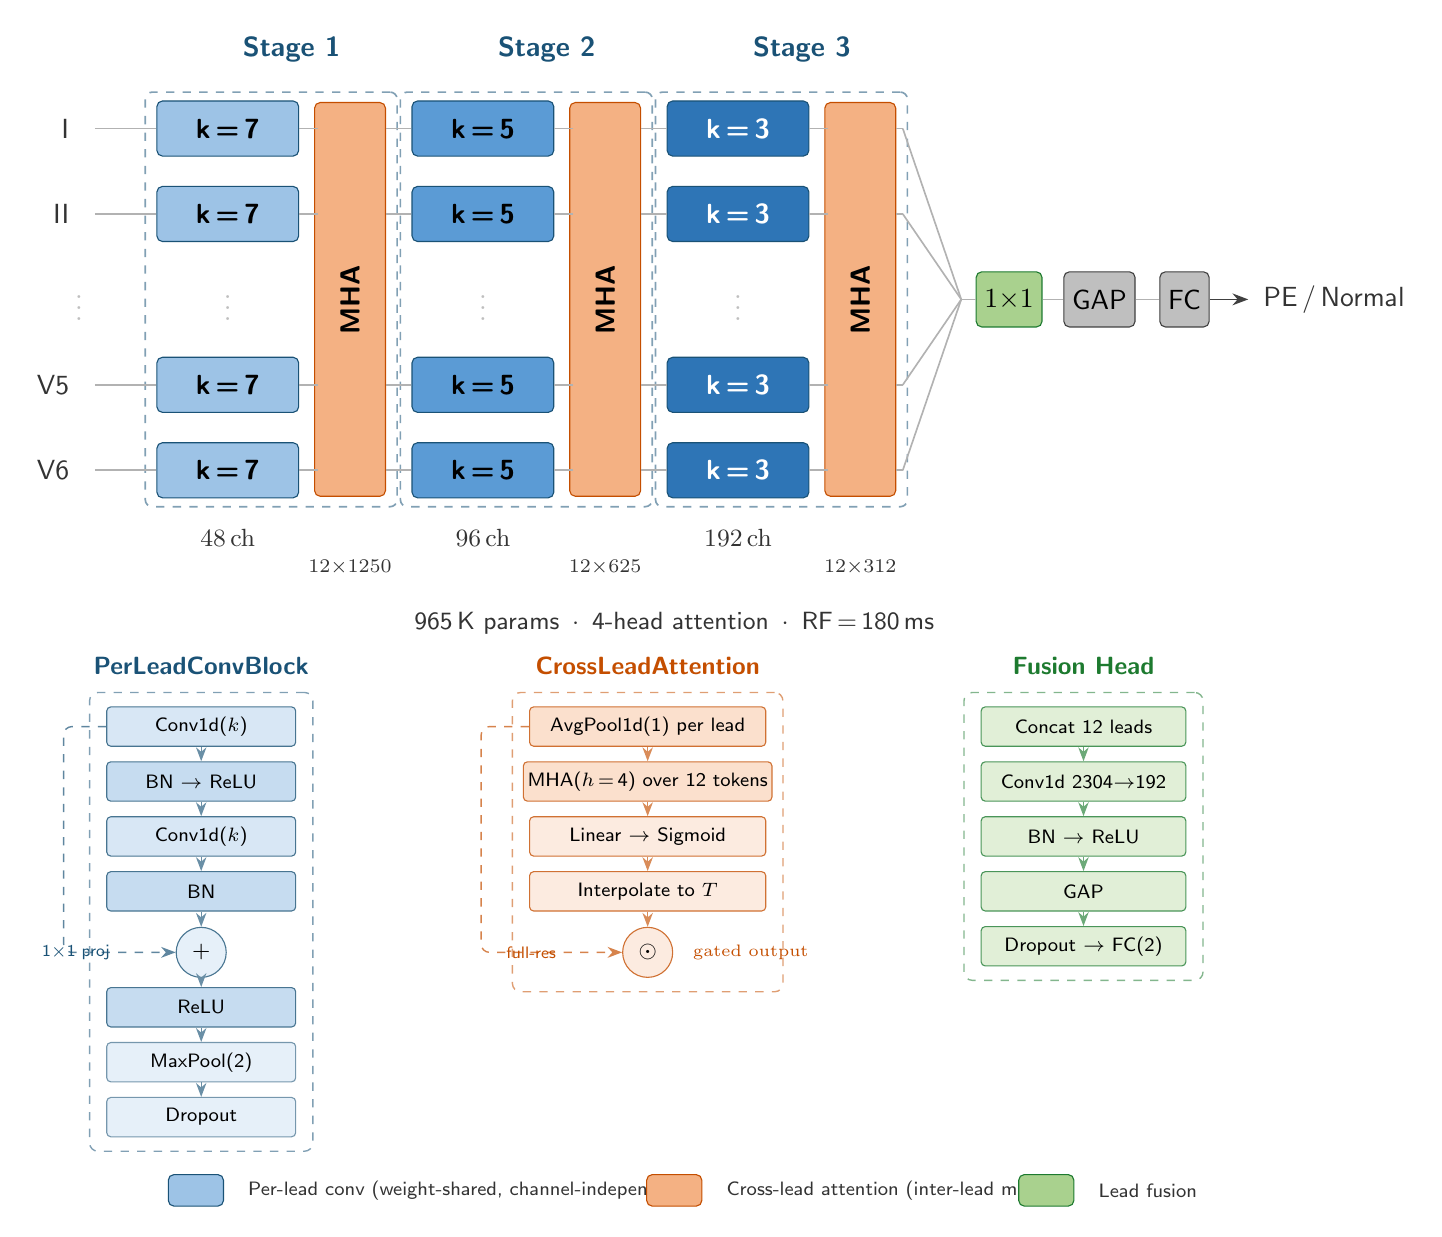
\begin{tikzpicture}[
  x=1.35cm, y=1.55cm,
  >=Stealth,
  cI/.style  ={rectangle, rounded corners=2pt,
               minimum width=18mm, minimum height=7mm,
               fill=stgI, draw=cdraw, line width=0.4pt,
               font=\normalsize\sffamily\bfseries, inner sep=2pt},
  cII/.style ={cI, fill=stgII},
  cIII/.style={cI, fill=stgIII, text=white},
  att/.style ={rectangle, rounded corners=2pt, minimum width=9mm,
               fill=afill, draw=adraw, line width=0.4pt,
               font=\normalsize\sffamily\bfseries, inner sep=2pt},
  fus/.style ={rectangle, rounded corners=2pt, minimum height=7mm,
               fill=ffill, draw=fdraw, line width=0.4pt,
               font=\normalsize\sffamily, inner sep=3pt},
  hd/.style  ={rectangle, rounded corners=2pt, minimum height=7mm,
               fill=hfill, draw=hdraw, line width=0.4pt,
               font=\normalsize\sffamily, inner sep=3pt},
  w/.style   ={draw=gray!60, line width=0.6pt},
  nt/.style  ={font=\small, text=notecol},
  sl/.style  ={font=\normalsize\sffamily\bfseries, text=cdraw},
  dm/.style  ={font=\scriptsize, text=notecol},
  detbox/.style={rectangle, rounded corners=2pt,
                 draw=cdraw!70, fill=stgI!18, line width=0.4pt,
                 inner sep=5pt, font=\small\sffamily,
                 text=notecol, align=left},
  detatt/.style={detbox, draw=adraw!70, fill=afill!18},
]

% ── Lead labels ──
\foreach \lid/\y/\nm in {a/1.4/I, b/0.7/II, c/-0.7/V5, d/-1.4/V6}{
  \node[font=\normalsize\sffamily, text=notecol, anchor=east]
    at (-0.1, \y) {\nm};
  \draw[w] (0.05, \y) -- (0.5, \y);
}
\node[font=\normalsize, text=gray!50] at (-0.1, 0) {$\vdots$};

% ── Stage 1: k=7, 48 ch ──
\foreach \lid/\y in {a/1.4, b/0.7, c/-0.7, d/-1.4}{
  \node[cI] (s1\lid) at (1.3, \y) {k\,=\,7};
  \draw[w] (0.5, \y) -- (s1\lid.west);
  \draw[w] (s1\lid.east) -- (2.15, \y);
}
\node[font=\normalsize, text=gray!50] at (1.3, 0) {$\vdots$};
\node[att, minimum height=50mm] (m1) at (2.45, 0)
  {\rotatebox{90}{\normalsize MHA}};
\foreach \y in {1.4, 0.7, -0.7, -1.4}{
  \draw[w] (2.15, \y) -- (m1.west |- 0,\y);
  \draw[w] (m1.east |- 0,\y) -- (2.85, \y);
}

% ── Stage 2: k=5, 96 ch ──
\foreach \lid/\y in {a/1.4, b/0.7, c/-0.7, d/-1.4}{
  \node[cII] (s2\lid) at (3.7, \y) {k\,=\,5};
  \draw[w] (2.85, \y) -- (s2\lid.west);
  \draw[w] (s2\lid.east) -- (4.55, \y);
}
\node[font=\normalsize, text=gray!50] at (3.7, 0) {$\vdots$};
\node[att, minimum height=50mm] (m2) at (4.85, 0)
  {\rotatebox{90}{\normalsize MHA}};
\foreach \y in {1.4, 0.7, -0.7, -1.4}{
  \draw[w] (4.55, \y) -- (m2.west |- 0,\y);
  \draw[w] (m2.east |- 0,\y) -- (5.25, \y);
}

% ── Stage 3: k=3, 192 ch ──
\foreach \lid/\y in {a/1.4, b/0.7, c/-0.7, d/-1.4}{
  \node[cIII] (s3\lid) at (6.1, \y) {k\,=\,3};
  \draw[w] (5.25, \y) -- (s3\lid.west);
  \draw[w] (s3\lid.east) -- (6.95, \y);
}
\node[font=\normalsize, text=gray!50] at (6.1, 0) {$\vdots$};
\node[att, minimum height=50mm] (m3) at (7.25, 0)
  {\rotatebox{90}{\normalsize MHA}};
\foreach \y in {1.4, 0.7, -0.7, -1.4}{
  \draw[w] (6.95, \y) -- (m3.west |- 0,\y);
  \draw[w] (m3.east |- 0,\y) -- (7.65, \y);
}

% ── Fusion head ──
\foreach \y in {1.4, 0.7, -0.7, -1.4}{
  \draw[w] (7.65, \y) -- (8.2, 0);
}
\node[fus] (f1) at (8.65, 0) {$1{\times}1$};
\draw[w] (8.2, 0) -- (f1.west);
\node[hd] (gap) at (9.5, 0) {GAP};
\draw[w] (f1.east) -- (gap.west);
\node[hd] (fc) at (10.3, 0) {FC};
\draw[w] (gap.east) -- (fc.west);
\draw[->, draw=hdraw, line width=0.6pt] (fc.east) -- (10.9, 0);
\node[nt, anchor=west, font=\normalsize\sffamily]
  at (10.95, 0) {PE\,/\,Normal};

% ── Stage labels ──
\node[sl] at (1.9,  2.05) {Stage 1};
\node[sl] at (4.3,  2.05) {Stage 2};
\node[sl] at (6.7,  2.05) {Stage 3};

% ── Channel counts + shapes ──
\node[nt] at (1.3,  -1.95) {48\,ch};
\node[nt] at (3.7,  -1.95) {96\,ch};
\node[nt] at (6.1,  -1.95) {192\,ch};
\node[dm] at (2.45, -2.2) {$12{\times}1250$};
\node[dm] at (4.85, -2.2) {$12{\times}625$};
\node[dm] at (7.25, -2.2) {$12{\times}312$};

\node[nt, font=\small\sffamily] at (5.5, -2.65)
  {965\,K params\enspace$\cdot$\enspace 4-head attention%
   \enspace$\cdot$\enspace RF\,=\,180\,ms};

% ════════════════════════════════════════════════════════════════════
%  DETAIL INSET — PerLeadConvBlock (mini flowchart with residual)
% ════════════════════════════════════════════════════════════════════
\begin{scope}[
  shift={(0.15, -3.35)},
  blk/.style={rectangle, rounded corners=1.5pt, minimum width=24mm,
              minimum height=5mm, draw=cdraw!80, fill=stgI!40,
              line width=0.4pt, font=\scriptsize\sffamily,
              inner sep=1.5pt},
  act/.style={blk, fill=stgII!35},
  pool/.style={blk, fill=stgI!25, draw=cdraw!60},
  add/.style={circle, minimum size=5.5mm, draw=cdraw!80, fill=stgI!25,
              line width=0.4pt, font=\footnotesize\sffamily\bfseries},
  arr/.style={draw=cdraw!65, line width=0.45pt, ->},
  skip/.style={draw=cdraw!70, line width=0.5pt, ->, rounded corners=3pt, dashed},
]
  \node[nt, font=\small\sffamily\bfseries, text=cdraw] at (0.9, 0.35) {PerLeadConvBlock};
  % main path
  \node[blk]  (cv1) at (0.9, -0.15) {Conv1d($k$)};
  \node[act]  (bn1) at (0.9, -0.6)  {BN $\to$ ReLU};
  \node[blk]  (cv2) at (0.9, -1.05) {Conv1d($k$)};
  \node[act]  (bn2) at (0.9, -1.5)  {BN};
  \node[add]  (res) at (0.9, -2.0)  {$+$};
  \node[act]  (rl2) at (0.9, -2.45) {ReLU};
  \node[pool] (mp)  at (0.9, -2.9)  {MaxPool(2)};
  \node[pool] (dp)  at (0.9, -3.35) {Dropout};
  % arrows
  \draw[arr] (cv1) -- (bn1);
  \draw[arr] (bn1) -- (cv2);
  \draw[arr] (cv2) -- (bn2);
  \draw[arr] (bn2) -- (res);
  \draw[arr] (res) -- (rl2);
  \draw[arr] (rl2) -- (mp);
  \draw[arr] (mp)  -- (dp);
  % residual skip
  \draw[skip] (cv1.west) -- ++(-0.4,0) |- node[pos=0.75, left,
    font=\fontsize{6}{7}\selectfont\sffamily, text=cdraw] {1$\times$1 proj} (res.west);
  % outer frame
  \node[draw=cdraw!55, dashed, line width=0.5pt, rounded corners=3pt,
    inner xsep=6pt, inner ysep=5pt,
    fit=(cv1)(dp)(res)] (dconv) {};
\end{scope}

% ════════════════════════════════════════════════════════════════════
%  DETAIL INSET — CrossLeadAttention (mini flowchart with gate)
% ════════════════════════════════════════════════════════════════════
\begin{scope}[
  shift={(4.15, -3.35)},
  blk/.style={rectangle, rounded corners=1.5pt, minimum width=30mm,
              minimum height=5mm, draw=adraw!80, fill=afill!40,
              line width=0.4pt, font=\scriptsize\sffamily,
              inner sep=1.5pt},
  gate/.style={blk, fill=afill!25},
  mul/.style={circle, minimum size=5.5mm, draw=adraw!80, fill=afill!25,
              line width=0.4pt, font=\footnotesize\sffamily\bfseries},
  arr/.style={draw=adraw!65, line width=0.45pt, ->},
  skip/.style={draw=adraw!70, line width=0.5pt, ->, rounded corners=3pt, dashed},
]
  \node[nt, font=\small\sffamily\bfseries, text=adraw] at (1.1, 0.35) {CrossLeadAttention};
  \node[blk]  (ap)  at (1.1, -0.15) {AvgPool1d(1) per lead};
  \node[blk]  (mha) at (1.1, -0.6)  {MHA($h$\,=\,4) over 12 tokens};
  \node[gate] (sig) at (1.1, -1.05) {Linear $\to$ Sigmoid};
  \node[gate] (int) at (1.1, -1.5)  {Interpolate to $T$};
  \node[mul]  (gm)  at (1.1, -2.0)  {$\odot$};
  % arrows
  \draw[arr] (ap)  -- (mha);
  \draw[arr] (mha) -- (sig);
  \draw[arr] (sig) -- (int);
  \draw[arr] (int) -- (gm);
  % bypass: full-res features
  \draw[skip] (ap.west) -- ++(-0.45,0) |- node[pos=0.8, left,
    font=\fontsize{6}{7}\selectfont\sffamily, text=adraw] {full-res} (gm.west);
  \node[nt, font=\fontsize{6}{7}\selectfont, text=adraw, anchor=west]
    at (gm.east) {\enspace gated output};
  % outer frame
  \node[draw=adraw!55, dashed, line width=0.5pt, rounded corners=3pt,
    inner xsep=6pt, inner ysep=5pt,
    fit=(ap)(gm)] (datt) {};
\end{scope}

% ════════════════════════════════════════════════════════════════════
%  DETAIL INSET — Fusion Head (mini flowchart)
% ════════════════════════════════════════════════════════════════════
\begin{scope}[
  shift={(8.35, -3.35)},
  blk/.style={rectangle, rounded corners=1.5pt, minimum width=26mm,
              minimum height=5mm, draw=fdraw!80, fill=ffill!35,
              line width=0.4pt, font=\scriptsize\sffamily,
              inner sep=1.5pt},
  arr/.style={draw=fdraw!65, line width=0.45pt, ->},
]
  \node[nt, font=\small\sffamily\bfseries, text=fdraw] at (1.0, 0.35) {Fusion Head};
  \node[blk] (cat)  at (1.0, -0.15) {Concat 12 leads};
  \node[blk] (c1x1) at (1.0, -0.6)  {Conv1d 2304$\to$192};
  \node[blk] (bn)   at (1.0, -1.05) {BN $\to$ ReLU};
  \node[blk] (gp)   at (1.0, -1.5)  {GAP};
  \node[blk] (drp)  at (1.0, -1.95) {Dropout $\to$ FC(2)};
  \draw[arr] (cat)  -- (c1x1);
  \draw[arr] (c1x1) -- (bn);
  \draw[arr] (bn)   -- (gp);
  \draw[arr] (gp)   -- (drp);
  \node[draw=fdraw!55, dashed, line width=0.5pt, rounded corners=3pt,
    inner xsep=6pt, inner ysep=5pt,
    fit=(cat)(drp)] (dfuse) {};
\end{scope}


% ── Legend ──
\node[cI,  minimum width=7mm, minimum height=4mm] at (1.0, -7.3) {};
\node[nt, anchor=west, font=\scriptsize\sffamily] at (1.4, -7.3)
  {Per-lead conv (weight-shared, channel-independent)};
\node[att, minimum width=7mm, minimum height=4mm] at (5.5, -7.3) {};
\node[nt, anchor=west, font=\scriptsize\sffamily] at (5.9, -7.3)
  {Cross-lead attention (inter-lead mixing)};
\node[fus, minimum width=7mm, minimum height=4mm] at (9.0, -7.3) {};
\node[nt, anchor=west, font=\scriptsize\sffamily] at (9.4, -7.3)
  {Lead fusion};

% ── Dashed stage groupings ──
\begin{scope}[on background layer]
  \node[draw=cdraw!55, dashed, line width=0.6pt, rounded corners=2.5pt,
    inner xsep=4pt, inner ysep=3pt,
    fit=(s1a)(s1d)(m1)] {};
  \node[draw=cdraw!55, dashed, line width=0.6pt, rounded corners=2.5pt,
    inner xsep=4pt, inner ysep=3pt,
    fit=(s2a)(s2d)(m2)] {};
  \node[draw=cdraw!55, dashed, line width=0.6pt, rounded corners=2.5pt,
    inner xsep=4pt, inner ysep=3pt,
    fit=(s3a)(s3d)(m3)] {};
\end{scope}

\end{tikzpicture}
\captionof{figure}{RepNet CrossLead 3-Stage architecture: per-lead 1D convolutions with shared weights alternate with 4-head cross-lead self-attention across three stages before fusion.}
\label{fig:arch}
\vspace{0.5em}
\end{strip}

\subsection{Channel Independent -- Shared Weights}

RepNet processes each lead through its own 1D convolutional stream with no cross-lead interaction until the attention step (\textit{channel-independent}). The question: does preeclampsia alter \textit{how leads relate to each other}, or \textit{what each lead looks like individually}?

We compute the $12 \times 12$ Pearson correlation matrix $C^{(n)}$ across leads for each recording $n$:
\begin{equation}
C^{(n)}_{ij} = \frac{\sum_{t=1}^{T} \bigl(x^{(n)}_{i,t} - \bar{x}^{(n)}_i\bigr)\bigl(x^{(n)}_{j,t} - \bar{x}^{(n)}_j\bigr)}{\sqrt{\sum_{t=1}^{T}\bigl(x^{(n)}_{i,t} - \bar{x}^{(n)}_i\bigr)^2}\;\sqrt{\sum_{t=1}^{T}\bigl(x^{(n)}_{j,t} - \bar{x}^{(n)}_j\bigr)^2}}
\end{equation}
where $x^{(n)}_{i,t}$ is the voltage of lead $i$ at time $t$. Averaging within each class:
\begin{equation}
\bar{C}_{\text{PE}} = \frac{1}{N_{\text{PE}}} \sum_{n \in \text{PE}} C^{(n)}, \qquad
\bar{C}_{\text{Normal}} = \frac{1}{N_{\text{Normal}}} \sum_{n \in \text{Normal}} C^{(n)}
\end{equation}

If preeclampsia disrupts inter-lead relationships, $\bar{C}_{\text{PE}} - \bar{C}_{\text{Normal}}$ would show large off-diagonal entries, favoring 2D convolution across leads. We quantify this with the Frobenius norm:
\begin{equation}
\| \bar{C}_{\text{PE}} - \bar{C}_{\text{Normal}} \|_F = \sqrt{\sum_{i=1}^{12}\sum_{j=1}^{12} \left(\bar{C}_{\text{PE},ij} - \bar{C}_{\text{Normal},ij}\right)^2} = 0.981
\end{equation}

\begin{figure}[H]
\centering

\includegraphics[width=\linewidth]{frobenius_diff.png}
\caption{Inter-lead correlation matrices for Normal ($N$\,=\,1843) and PreE ($N$\,=\,335) classes, and their difference.}
\label{fig:frobenius}
\end{figure}

As shown in Figure~\ref{fig:frobenius}, the two matrices are nearly identical. The difference matrix has maximum entries below $\pm 0.18$, and the Frobenius norm of 0.981 is well below the 2.0 threshold for clinically meaningful disruption. The discriminative signal is within each lead's waveform (ST/T-wave morphology), not in inter-lead coupling. This justifies per-lead 1D convolution.

RepNet uses shared weights: one CNN applied identically to every lead, rather than 12 independent CNNs. Two reasons:
\begin{enumerate}
\item \textbf{Shared structure.} All 12 leads record the same heartbeat, differing only in amplitude/polarity due to the cardiac axis. The same convolutional filters are useful across all leads.
\item \textbf{Data multiplication.} With 335 PE recordings, independent weights per lead see 335 examples each. Shared weights see $335 \times 12 = 4{,}020$ lead-level examples --- critical regularization in a data-limited regime.
\end{enumerate}

The trade-off --- shared weights cannot learn lead-specific features --- is handled by the cross-lead attention mechanism, which learns to weight leads differently after per-lead features are extracted.

\subsection{Three-Stage Progressive Abstraction}

RepNet processes each lead through three convolutional stages with doubling filter counts (48$\to$96$\to$192) and shrinking kernel sizes (7$\to$5$\to$3). MaxPool(2) halves the temporal axis at each stage: $2500 \to 1250 \to 625 \to 312$ samples. Table~\ref{tab:arch} summarizes the architecture.

\begin{table}[H]
\centering
\caption{RepNet CrossLead 3-Stage architecture summary.}
\label{tab:arch}
\small
\begin{tabular}{lcccc}
\toprule
 & \textbf{Filters} & \textbf{Kernel} & \textbf{Output Shape} & \textbf{Attention} \\
\midrule
Input          & ---  & ---  & $12 \times 2500$ & ---        \\
Stage 1        & 48   & k=7  & $12 \times 1250$ & 4-head MHA \\
Stage 2        & 96   & k=5  & $12 \times 625$  & 4-head MHA \\
Stage 3        & 192  & k=3  & $12 \times 312$  & 4-head MHA \\
Fusion ($1\!\times\!1$) & 192  & k=1  & $1 \times 312$   & ---        \\
GAP            & ---  & ---  & 192              & ---        \\
FC             & ---  & ---  & 2 (softmax)      & ---        \\
\bottomrule
\end{tabular}
\end{table}

The design rationale is frequency-driven. Wider kernels at early stages capture broad morphological features (QRS complex) on raw 250\,Hz signals. Narrower kernels at deeper stages refine on already-downsampled representations where each sample spans a larger temporal window. Each PerLeadConvBlock contains two same-padded convolutions followed by MaxPool(2). Treating the pool as a stride-only operation, the receptive field at stage $s$ accumulates as:
\begin{equation}
\text{RF}_s = \text{RF}_{s-1} + 2\,(k_s - 1) \cdot \prod_{j=1}^{s-1} 2
\end{equation}
where the factor of 2 inside the product is the pool stride per stage. Expanding for three stages:
\begin{align}
\text{RF} &= 1 + 2(k_1{-}1)\cdot 1 + 2(k_2{-}1)\cdot 2 + 2(k_3{-}1)\cdot 4 \notag \\
           &= 2k_1 + 4k_2 + 8k_3 - 13 \notag \\
           &= 2(7) + 4(5) + 8(3) - 13 = 45 \text{ samples} = 180\text{\,ms}
\end{align}
This covers the QRS complex (80--120\,ms) and extends into the ST segment, where preeclampsia's primary ECG signature --- mild repolarization abnormalities --- resides. The GAP layer in the fusion head subsequently collapses the full remaining temporal dimension, giving the classifier access to the entire 10\,s recording.

Table~\ref{tab:rf-search} shows the Optuna kernel search over 20 trials across 8 unique configurations.

\begin{table}[H]
\centering
\caption{Optuna kernel/receptive-field search: best CV AUROC per configuration.}
\label{tab:rf-search}
\small
\begin{tabular}{lcrc}
\toprule
\textbf{Kernels} & \textbf{RF (samples)} & \textbf{RF (ms)} & \textbf{Best CV AUROC} \\
\midrule
(3, 3, 3)    & 29  & 116  & 0.6815 \\
(5, 3, 3)    & 33  & 132  & 0.6925 \\
(5, 5, 3)    & 41  & 164  & 0.6792 \\
(7, 5, 3)    & 45  & 180  & \textbf{0.7022} \\
(9, 5, 3)    & 49  & 196  & 0.6712 \\
(9, 7, 5)    & 73  & 292  & 0.6938 \\
(11, 7, 5)   & 77  & 308  & 0.6649 \\
(13, 9, 5)   & 89  & 356  & 0.6867 \\
\bottomrule
\end{tabular}
\end{table}

The $(7,5,3)$ configuration at RF\,=\,180\,ms achieved the best CV AUROC of 0.7022 (test AUROC 0.7817). Performance peaks in the 130--180\,ms range and degrades on both sides. Configurations below 130\,ms --- such as $(3,3,3)$ at 116\,ms --- cannot span the full QRS complex, missing the morphological context needed for classification. Configurations above 200\,ms --- such as $(11,7,5)$ at 308\,ms or $(13,9,5)$ at 356\,ms --- use wider kernels that increase parameter count without benefit, as the additional temporal context (T-wave tail, baseline) adds noise rather than discriminative signal. The $(9,7,5)$ triple at 292\,ms is a notable exception (0.6938), likely because its balanced kernel progression still captures the QRS--ST window effectively despite the excess reach. The sweet spot at 180\,ms aligns with the QRS onset through early T-wave, which is precisely where preeclampsia-related repolarization abnormalities manifest.

\subsection{Cross-Lead Attention Mechanism}

After each per-lead convolutional stage, a cross-lead attention block allows the 12 leads to exchange information. The mechanism operates as follows:
\begin{enumerate}
\item \textbf{Tokenization.} Each lead's feature map $(C \times T)$ is pooled to a single $C$-dimensional vector via AdaptiveAvgPool1d(1), yielding 12 tokens.
\item \textbf{Self-attention.} 4-head multi-head attention operates over the 12 lead-tokens with residual connection and LayerNorm.
\item \textbf{Gating.} The attended representation passes through a linear layer and sigmoid to produce per-lead gate weights in $[0, 1]$. These weights are broadcast back to the full temporal resolution and applied element-wise: $\mathbf{x}_\ell' = \sigma(\mathbf{g}_\ell) \odot \mathbf{x}_\ell$.
\end{enumerate}

The gating design is deliberate. Rather than replacing each lead's features with the attention output, the gate \textit{modulates} the original full-resolution features. Leads deemed uninformative by attention are suppressed; informative leads are amplified. This preserves temporal detail that would be lost if the pooled attention output were used directly.

Attention is placed between every convolutional stage (three attention blocks total), not only at the end. This allows cross-lead context to inform feature extraction at each abstraction level: QRS-level (Stage~1), ST-level (Stage~2), and morphology-level (Stage~3).

Compared to 2D convolution across leads, attention preserves lead identity throughout the network and produces interpretable per-lead weights that can be analyzed post hoc to determine which leads the model relies on for classification. Figure~\ref{fig:attention} shows the mean $12 \times 12$ attention matrices across the test set, separated by class.

Stage~1 attention is nearly perfectly uniform (deviations $< 0.1\%$ from $1/12$), confirming that early-stage features are not yet class-discriminative. Stages~2 and~3 develop \textit{vertical striping}: entire columns are consistently brighter or darker regardless of the query row. This key-dominated pattern means the model has learned \textit{which leads are worth listening to} rather than pairwise lead relationships --- every lead looks to the same informative sources.

The column structure is consistent across both classes: aVR and V1 are suppressed ($\sim$0.6--0.9\% below uniform), while lateral leads V5, V6, II, and aVF are boosted ($\sim$0.3--0.4\% above uniform). This aligns with clinical expectations --- aVR is an inverted view of the heart that rarely carries primary diagnostic information, while the lateral and inferior leads are most sensitive to the repolarization abnormalities associated with preeclampsia. Class-level differences are subtle ($<$0.03\% of uniform) but structured: in Stage~2, PE samples attend more to aVL and Lead~I (the high-lateral leads) and less to V2--V3, consistent with left-axis-directed repolarization changes. These small attention shifts are amplified by the multiplicative sigmoid gate acting on full-resolution feature maps.

\begin{figure}[H]
\centering
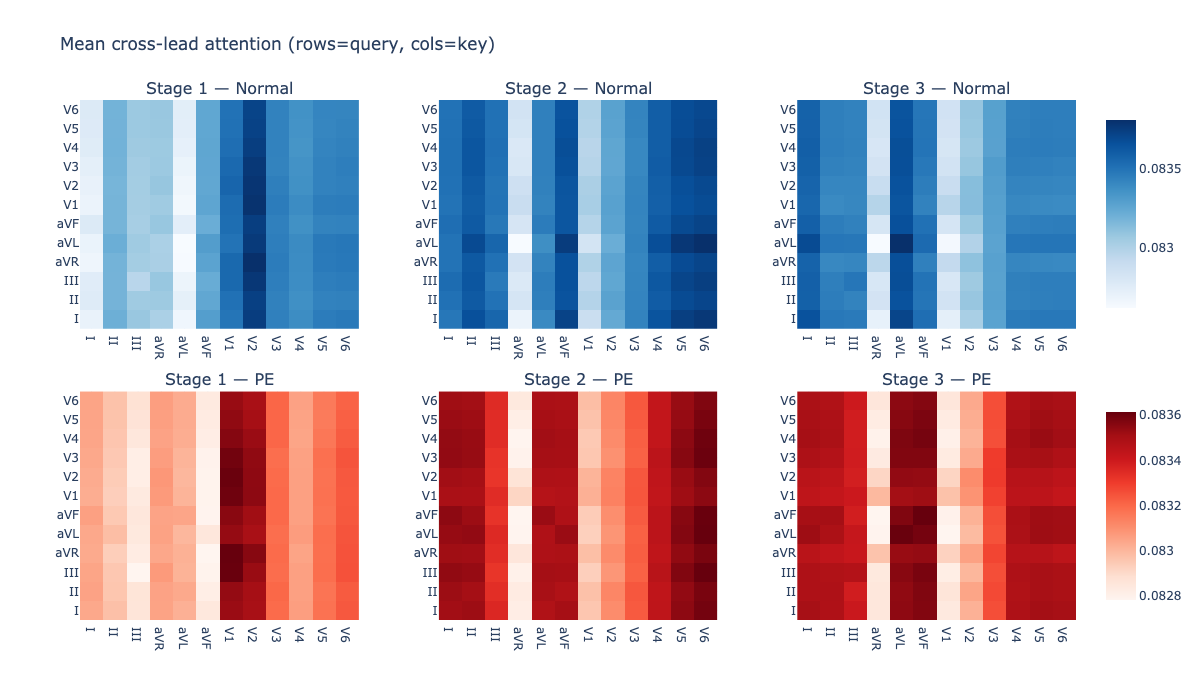
\includegraphics[width=\linewidth]{fig_attention_final.png}
\caption{Mean cross-lead attention matrices (rows = query lead, columns = key lead) for Normal (top) and PE (bottom) across three stages.}
\label{fig:attention}
\end{figure}

\subsection{Fusion Head and Classification}

The fusion head is the only component where all 12 leads merge into a single representation. After Stage~3, the 12 lead feature maps are concatenated along the channel axis: $(B, 12, 192, 312) \to (B, 2304, 312)$. A pointwise $1
\times 1$ convolution reduces this to $(B, 192, 312)$ with BatchNorm and ReLU, forcing the network to learn a compact cross-lead representation rather than retaining all $12 \times 192 = 2304$ channels. Global average pooling (GAP) then collapses the temporal axis to a 192-dimensional vector. Dropout followed by a fully-connected layer produces the 2-class output (PE vs.\ Normal).

The 1x1 convolution is preferred over flattening for parameter efficiency: flattening $2304 \times 312$ directly into a classifier would require over 700K parameters in the FC layer alone. The pointwise conv uses only $2304 \times 192 = 442$K parameters and preserves the temporal structure for GAP.

The final classification reduces to a 192-channel vote. Each GAP channel $i$ contributes a vote $v_i = \text{GAP}_i \cdot (W_{\text{PE},i} - W_{\text{Normal},i})$ to the PE-vs-Normal decision margin; the sum of all votes plus a bias term passes through softmax. Figure~\ref{fig:voting} visualizes this mechanism. The structural weights (top) show which channels are wired toward PE (positive) or Normal (negative). The per-sample panels show a confident true positive (margin $= +1.24$, PE votes dominate) and a confident true negative (margin $= -4.28$, Normal votes dominate).

\begin{figure}[H]
\centering
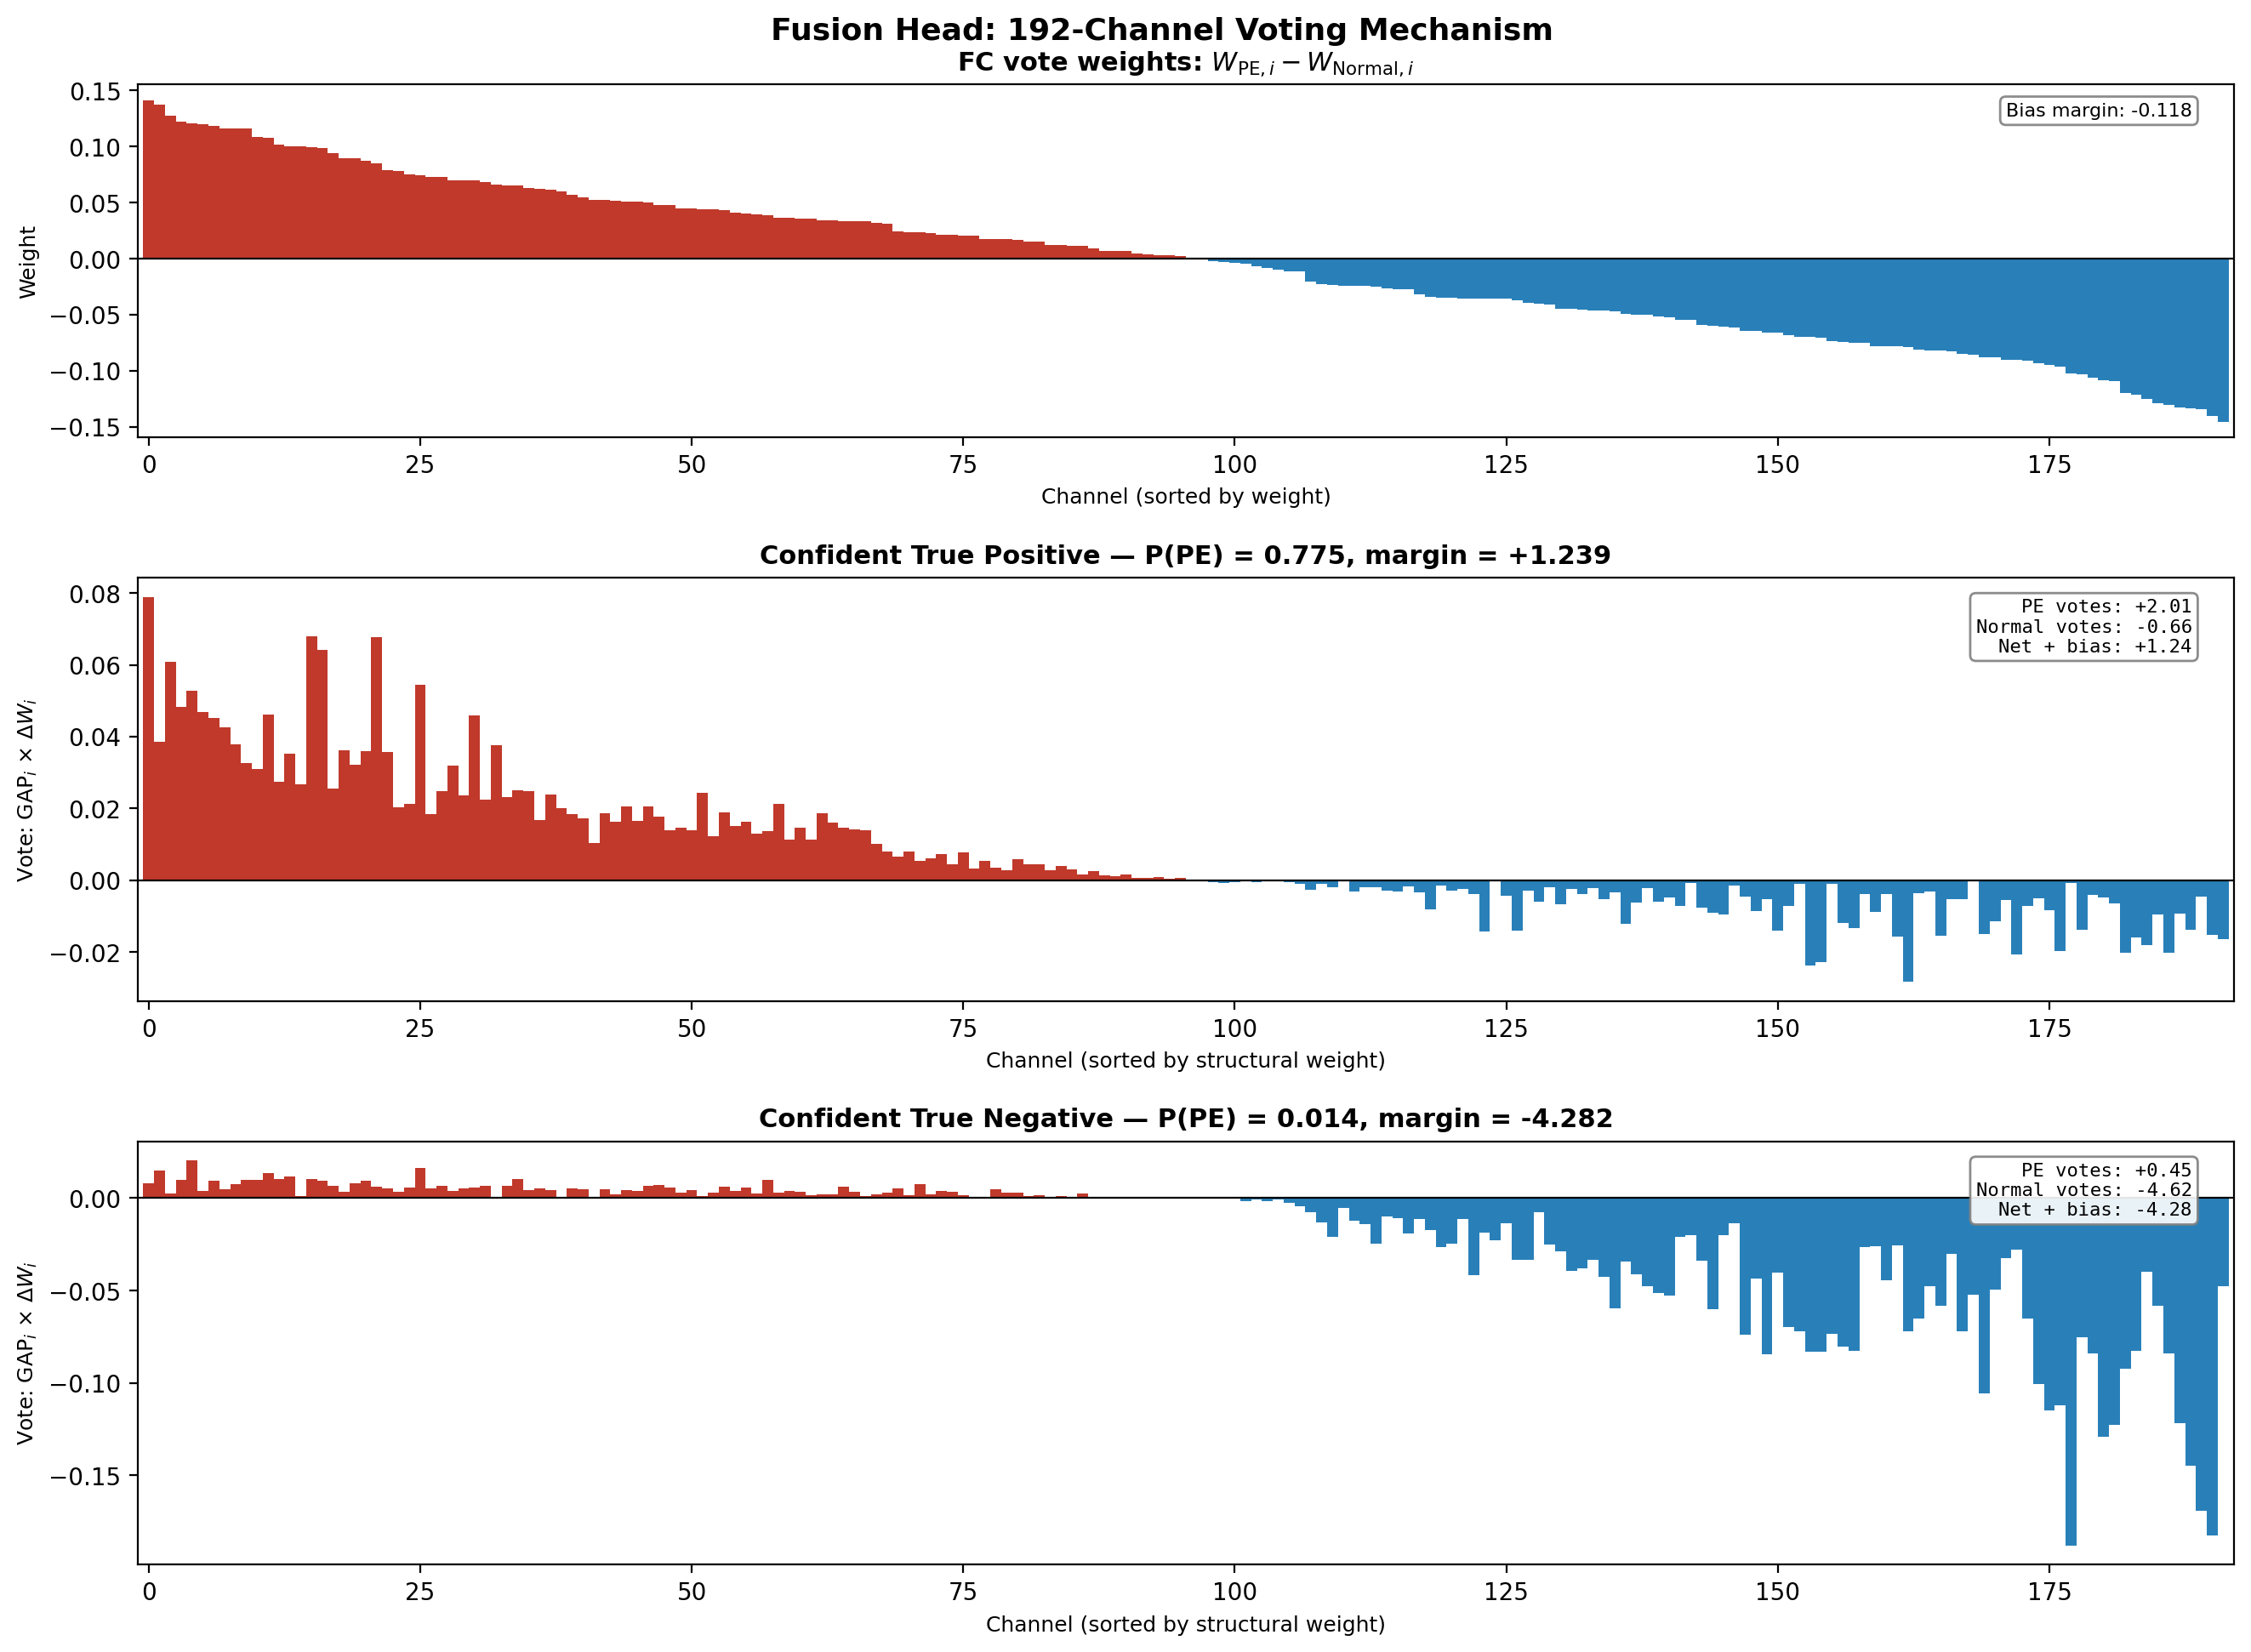
\includegraphics[width=\linewidth]{fig_voting.png}
\caption{192-channel voting mechanism. Top: FC vote weights. Middle/bottom: per-channel vote contributions for a confident TP and TN.}
\label{fig:voting}
\end{figure}

\subsubsection{Parameter Budget and Capacity Analysis}

The finalized model has 965K parameters, selected by Optuna's filter search over 30 trials across eight filter configurations ranging from 27K to 965K parameters. Table~\ref{tab:filter-search} summarizes the results.

\begin{table}[H]
\centering
\caption{Optuna filter search: best CV AUROC per configuration.}
\label{tab:filter-search}
\small
\begin{tabular}{lrr}
\toprule
\textbf{Filters} & \textbf{Params} & \textbf{Best CV AUROC} \\
\midrule
(8, 16, 32)    & 27K   & 0.6826 \\
(16, 32, 64)   & 108K  & 0.6650 \\
(32, 32, 64)   & 120K  & 0.6731 \\
(16, 32, 96)   & 215K  & 0.6969 \\
(16, 48, 96)   & 236K  & 0.6907 \\
(24, 48, 96)   & 242K  & 0.6718 \\
(32, 64, 128)  & 430K  & 0.6835 \\
(48, 96, 192)  & 965K  & \textbf{0.7034} \\
\bottomrule
\end{tabular}
\end{table}

The key observation: all configurations converge to a narrow CV AUROC band of 0.66--0.70. The 965K model wins, but the 27K model (36$\times$ smaller) scores within 0.021. This is a \textit{data-limited} regime, not a capacity-limited one --- with only 335 PE recordings, adding parameters yields diminishing returns because the model cannot see enough pathological variation to exploit extra capacity.

Multi-seed validation (30 independent runs with the 965K configuration) confirms this: mean AUROC = $0.7443 \pm 0.054$, with individual seeds ranging from 0.6153 to 0.8205. The high variance across seeds further indicates data limitation rather than architectural insufficiency.

\section{Dataset and Preprocessing}

\subsection{UC Davis Health ECG Dataset}

The dataset consists of 12-lead ECG recordings from UC Davis Health, sampled at 250\,Hz for 10\,s (2500 samples per lead). Each recording is stored as a CSV with shape $12 \times 2500$. Table~\ref{tab:dataset} summarizes the class distribution.

\begin{table}[H]
\centering
\caption{UC Davis Health preeclampsia ECG dataset.}
\label{tab:dataset}
\small
\begin{tabular}{lrr}
\toprule
 & \textbf{Patients} & \textbf{ECGs} \\
\midrule
Normal     & 1{,}217 & 1{,}854 \\
Preeclampsia & 132   & 187 \\
\midrule
\textbf{Total} & 1{,}349 & 2{,}041 \\
Ratio (Normal\,:\,PE) & \multicolumn{2}{c}{$\sim$9.9\,:\,1} \\
\bottomrule
\end{tabular}
\end{table}

The dataset is severely imbalanced: Normal ECGs outnumber PE recordings by nearly 10:1. Some patients contribute multiple ECGs, creating a risk of data leakage if the same patient appears in both training and test sets.

\subsection{Preprocessing Pipeline}

Three preprocessing steps are applied in order:
\begin{enumerate}
\item \textbf{Baseline wander removal.} A 4th-order Butterworth high-pass filter at 0.5\,Hz, the clinical standard cutoff for ECG baseline correction (cite), removes slow electrode drift. Implemented in SOS (second-order sections) form for numerical stability.
\item \textbf{Powerline interference removal.} A notch filter at 60\,Hz ($Q = 30$) suppresses US power grid interference. The narrow $Q$ factor limits the notch width to $\sim$1\,Hz, preserving signal content near 60\,Hz.
\item \textbf{Z-score normalization.} Each lead is independently normalized to zero mean and unit variance: $(x - \mu_\ell) / (\sigma_\ell + \epsilon)$, $\epsilon = 10^{-8}$. Per-lead normalization preserves amplitude differences between leads that encode cardiac axis information.
\end{enumerate}

Figure~\ref{fig:preprocessing} illustrates each step on a synthetic ECG waveform.

\begin{figure}[H]
\centering
\begin{tikzpicture}
\begin{groupplot}[
  group style={
    group size=2 by 2,
    horizontal sep=1.2cm,
    vertical sep=0.8cm,
  },
  width=0.52\columnwidth,
  height=2.4cm,
  domain=0:1.6,
  samples=200,
  grid=none,
  axis lines=left,
  tick label style={font=\scriptsize},
  title style={font=\small\bfseries},
  xtick=\empty,
  ytick style={draw=none},
  every axis plot/.style={draw=stgIII, line width=0.5pt, no markers, smooth},
]

\nextgroupplot[
  title={1.\ Raw ECG},
  ymin=-0.8, ymax=1.8,
  ytick={-0.5, 0, 0.5, 1.0, 1.5},
  ylabel={\scriptsize mV},
]
\addplot {ecgsig(x)+0.6*sin(deg(2*3.14159*0.5*x))+0.06*sin(deg(2*3.14159*15*x))};

\nextgroupplot[
  title={2.\ Baseline Removed},
  ymin=-0.6, ymax=1.5,
  ytick={0, 0.5, 1.0},
]
\addplot {ecgsig(x)+0.06*sin(deg(2*3.14159*15*x))};

\nextgroupplot[
  title={3.\ 60\,Hz Notch},
  ymin=-0.6, ymax=1.5,
  ytick={0, 0.5, 1.0},
  ylabel={\scriptsize mV},
  xtick={0, 0.5, 1.0, 1.5},
  xlabel={\scriptsize s},
]
\addplot {ecgsig(x)};

\nextgroupplot[
  title={4.\ Z-score},
  ymin=-1.5, ymax=4.0,
  ytick={-1, 0, 1, 2, 3},
  ylabel={\scriptsize $\sigma$},
  xtick={0, 0.5, 1.0, 1.5},
  xlabel={\scriptsize s},
]
\addplot {(ecgsig(x)-0.08)/0.3};

\end{groupplot}
\end{tikzpicture}
\caption{Preprocessing pipeline illustrated on a synthetic ECG: (1) raw signal with baseline wander and powerline noise, (2) after 0.5\,Hz highpass, (3) after 60\,Hz notch filter, (4) after per-lead z-score normalization.}
\label{fig:preprocessing}
\end{figure}

Quality filtering removes 8 recordings with flat leads (std $< 10^{-4}$) and 5 with missing patient identifiers, yielding 2{,}028 usable recordings.

\subsection{Data Split and Balancing}

An 80/20 patient-grouped holdout split ensures no patient appears in both dev and test sets. The dev set contains 1{,}747 recordings (15.9\% PE); the test set contains 431 recordings (13.5\% PE). The test set is never balanced, preserving clinical prevalence for evaluation.

Within the dev set, training data is balanced via symmetric augmentation followed by majority undersampling. Both PE and Normal samples are augmented with Gaussian noise ($\sigma = 0.06$) and random time shifts (up to $\pm 276$ samples $\approx \pm 1.1$\,s), doubling each class. Majority undersampling then reduces the Normal class to match PE count, yielding a 1:1 training ratio. Because the Normal class is undersampled after doubling, the final training set contains a fair mix of original and augmented Normal waveforms rather than being entirely synthetic. Augmenting both classes symmetrically prevents the model from learning augmentation artifacts as class-discriminative features.

\section{Model Meta-Analysis}

The 192-dimensional GAP embedding produced by RepNet's penultimate layer provides a rich space for post-hoc analysis of what the model has learned, where it fails, and how its decision landscape is structured. All analyses in this section use the best single seed (seed \#49, test AUROC = 0.8205) with PCA fit on the development set to avoid leakage.

\subsection{Embedding Geometry}

Dimensionality reduction of the 192-d GAP embeddings confirms that the ECG carries a learnable preeclampsia signal. We apply two complementary projections. PCA (principal component analysis) finds the linear axes of greatest variance, preserving global structure. t-SNE (t-distributed stochastic neighbor embedding) is a nonlinear method that optimizes a probabilistic mapping to preserve local neighborhood structure --- points close in 192-d stay close in 2-d, revealing clusters and manifold geometry that linear projections miss.

Both projections (Figures~\ref{fig:pca_class}--\ref{fig:tsne_prob}) show PE samples concentrating in a distinct region of embedding space, separated from the bulk Normal population. The model's predicted $P(\text{PE})$ tracks this geometry closely: high-confidence predictions (red) align with the PE cluster while low-confidence predictions (blue) align with the Normal cluster, producing a visible decision boundary with a gradient transition zone where the two classes overlap. The t-SNE projection reveals tighter cluster structure than PCA, with a geometrically distinct high-confidence Normal cluster that is not simply a linear tail of the distribution.

The representation is also highly compressed. The first 5 principal components capture 87.8\% of variance, and the channel correlation matrix has an effective rank of 6.0 --- the 192-channel GAP layer encodes approximately 6 independent dimensions of variation. A linear probe on just 7 PCs matches the full nonlinear model's test AUROC (0.826 vs.\ 0.821), indicating that the discriminative signal is low-dimensional and approximately linear in the learned feature space.

\begin{figure}[H]
\centering
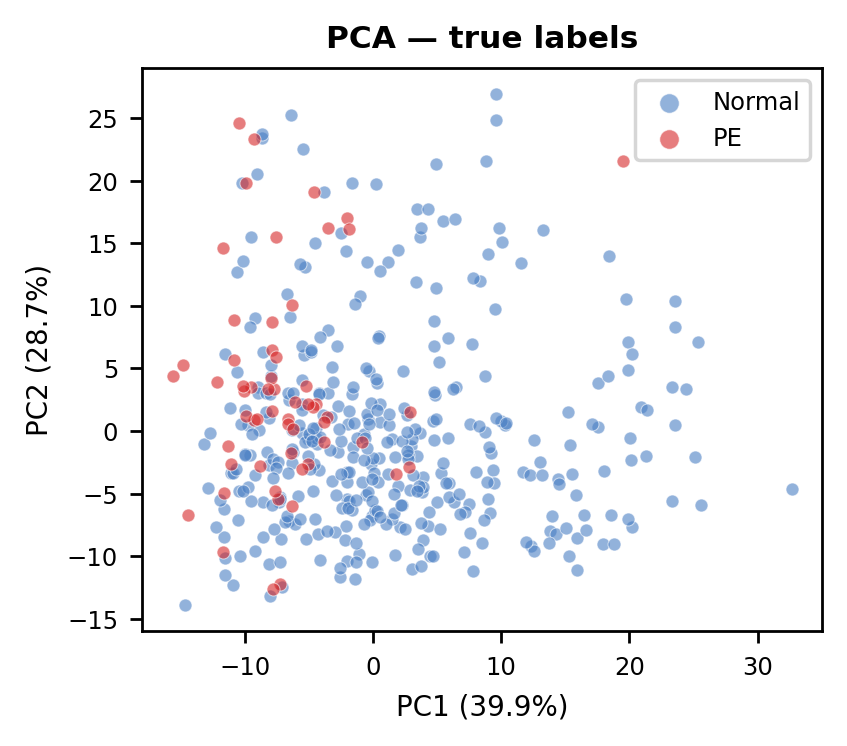
\includegraphics[width=\columnwidth]{fig_pca_class.png}
\caption{PCA projection of 192-d GAP embeddings colored by true class. Normal samples concentrate at positive PC1; PE samples shift toward negative PC1.}
\label{fig:pca_class}
\end{figure}

\begin{figure}[H]
\centering
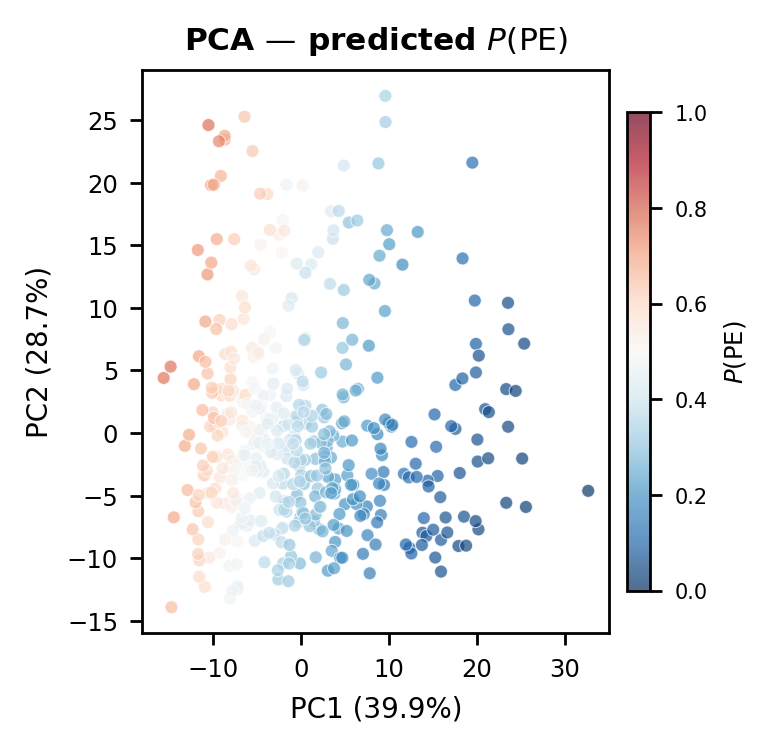
\includegraphics[width=\columnwidth]{fig_pca_prob.png}
\caption{PCA projection colored by predicted $P(\text{PE})$. The blue-to-red gradient traces the decision boundary through the class-overlap zone.}
\label{fig:pca_prob}
\end{figure}

\begin{figure}[H]
\centering
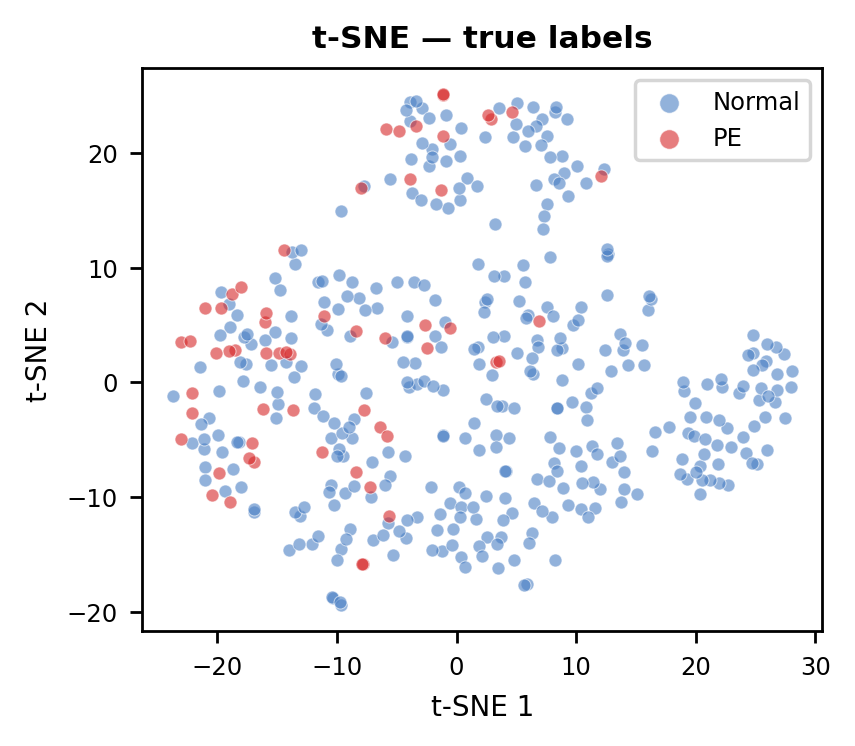
\includegraphics[width=\columnwidth]{fig_tsne_class.png}
\caption{t-SNE projection colored by true class. Nonlinear embedding reveals tighter cluster structure than PCA.}
\label{fig:tsne_class}
\end{figure}

\begin{figure}[H]
\centering
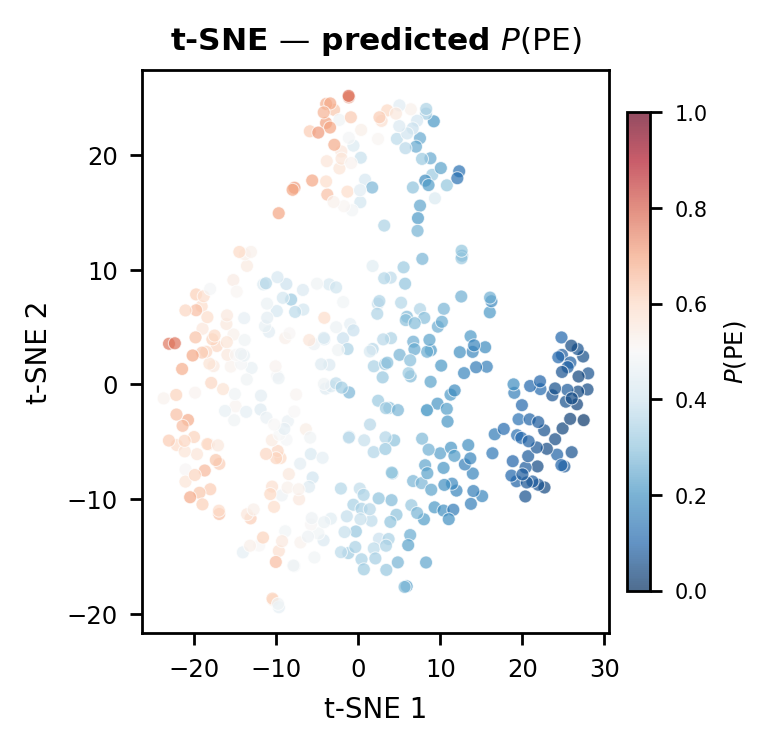
\includegraphics[width=\columnwidth]{fig_tsne_prob.png}
\caption{t-SNE projection colored by predicted $P(\text{PE})$. High-confidence Normal cluster (blue) is geometrically distinct from the PE region (red).}
\label{fig:tsne_prob}
\end{figure}

The projections confirm that the model has learned a meaningful decision boundary: PE samples occupy a distinct region of the embedding space, and the predicted probability gradient aligns with the geometric separation between classes. However, substantial overlap remains --- particularly in the transition zone where Normal-high and PE-low samples intermingle. This overlap is consistent with the model's 89 false positives and 18 false negatives at $\tau{=}0.5$, and reflects the fundamental difficulty of the task: with only 335 PE recordings and subtle morphological differences between classes, the ECG signal alone does not permit clean separation. Reducing this overlap will likely require either additional training data or complementary clinical features beyond the raw waveform.

\subsection{Classification Performance}

Table~\ref{tab:classification} reports classification metrics for the best single seed (\#49) and the 30-seed distribution. All threshold-dependent metrics use $\tau{=}0.5$.

\begin{table}[H]
\centering
\caption{Classification performance on the held-out test set ($n{=}431$: 373 Normal, 58 PE). Threshold-dependent metrics evaluated at $\tau{=}0.5$.}
\label{tab:classification}
\small
\begin{tabular}{lccc}
\toprule
Metric & Best seed & Mean $\pm$ SD & Range \\
\midrule
AUROC       & 0.821 & $0.744 \pm 0.053$ & 0.615--0.821 \\
AUPRC       & 0.429 & $0.312 \pm 0.061$ & 0.186--0.429 \\
Sensitivity & 0.690 & $0.624 \pm 0.263$ & 0.121--1.000 \\
Specificity & 0.761 & $0.676 \pm 0.201$ & 0.220--0.968 \\
Precision   & 0.310 & $0.264 \pm 0.065$ & 0.166--0.423 \\
Accuracy    & 0.752 & $0.669 \pm 0.142$ & 0.325--0.856 \\
F1-score    & 0.428 & $0.331 \pm 0.057$ & 0.182--0.441 \\
\bottomrule
\end{tabular}
\end{table}

The best seed achieves an AUROC of 0.821 and sensitivity of 0.690 at a specificity of 0.761, but these numbers overstate expected performance. The 30-seed distribution reveals substantial variance: sensitivity ranges from 0.121 to 1.000 (SD = 0.263) and specificity from 0.220 to 0.968 (SD = 0.201), reflecting instability in the decision boundary across random initializations.

The low precision (0.310) is a direct consequence of the 6.4:1 class imbalance in the test set: even with 76\% specificity, the 373 Normal samples produce 89 false positives that outnumber the 40 true positives. At a sensitivity target of $\geq$0.90 (clinically relevant for screening), the required threshold drops to $\tau{=}0.449$, yielding specificity of 0.673 and precision of 0.303 --- 53 of 58 PE cases are captured, but at the cost of flagging 122 Normal patients.

Figure~\ref{fig:roc_pr} shows the ROC and precision-recall curves for the best seed. The precision-recall curve highlights the challenge posed by low prevalence: precision drops steeply as recall increases beyond 0.5, and the area under the PR curve (0.429) reflects the difficulty of achieving high positive predictive value with a 13.5\% base rate.

\begin{figure}[H]
\centering
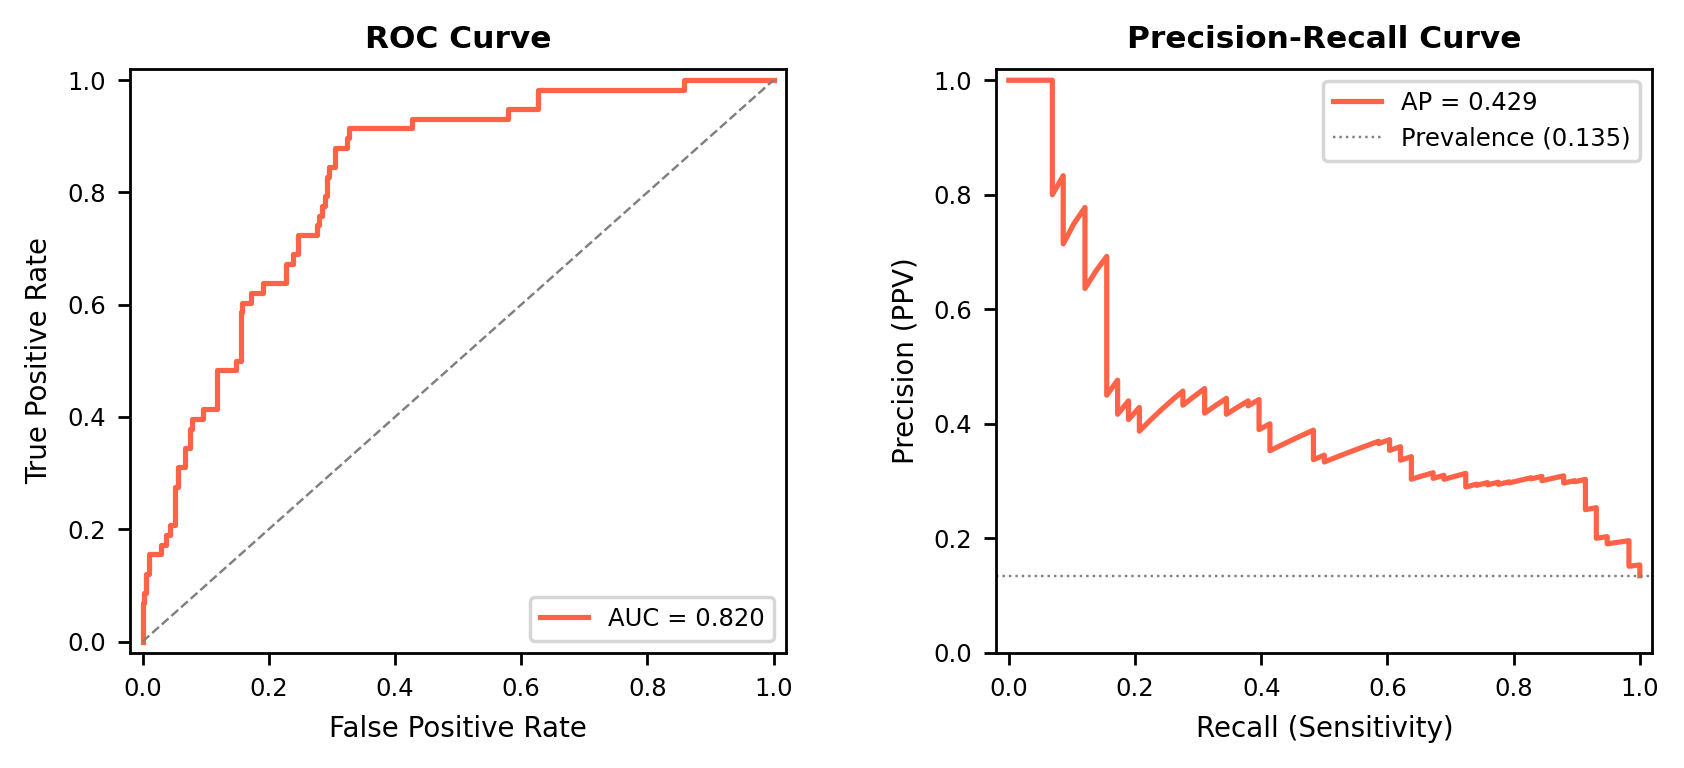
\includegraphics[width=\columnwidth]{fig_roc_pr.png}
\caption{ROC and precision-recall curves for the best seed on the test set.}
\label{fig:roc_pr}
\end{figure}

Figure~\ref{fig:pred_youden}(a) shows the distribution of predicted probabilities by true class. The Normal distribution is broad and left-shifted but extends well past $\tau{=}0.5$, producing the 89 false positives. The PE distribution is right-shifted but heavily overlaps with Normal in the 0.2--0.6 range. Figure~\ref{fig:pred_youden}(b) shows the Youden's $J$ statistic ($J = \text{sensitivity} + \text{specificity} - 1$) as a function of threshold. The optimal threshold $\tau^*{=}0.448$ ($J{=}0.587$) is close to the default $\tau{=}0.5$, with sensitivity of 0.914 and specificity of 0.673 --- a favorable trade-off for screening where missing PE cases carries higher clinical cost than false alarms.

\begin{figure}[H]
\centering
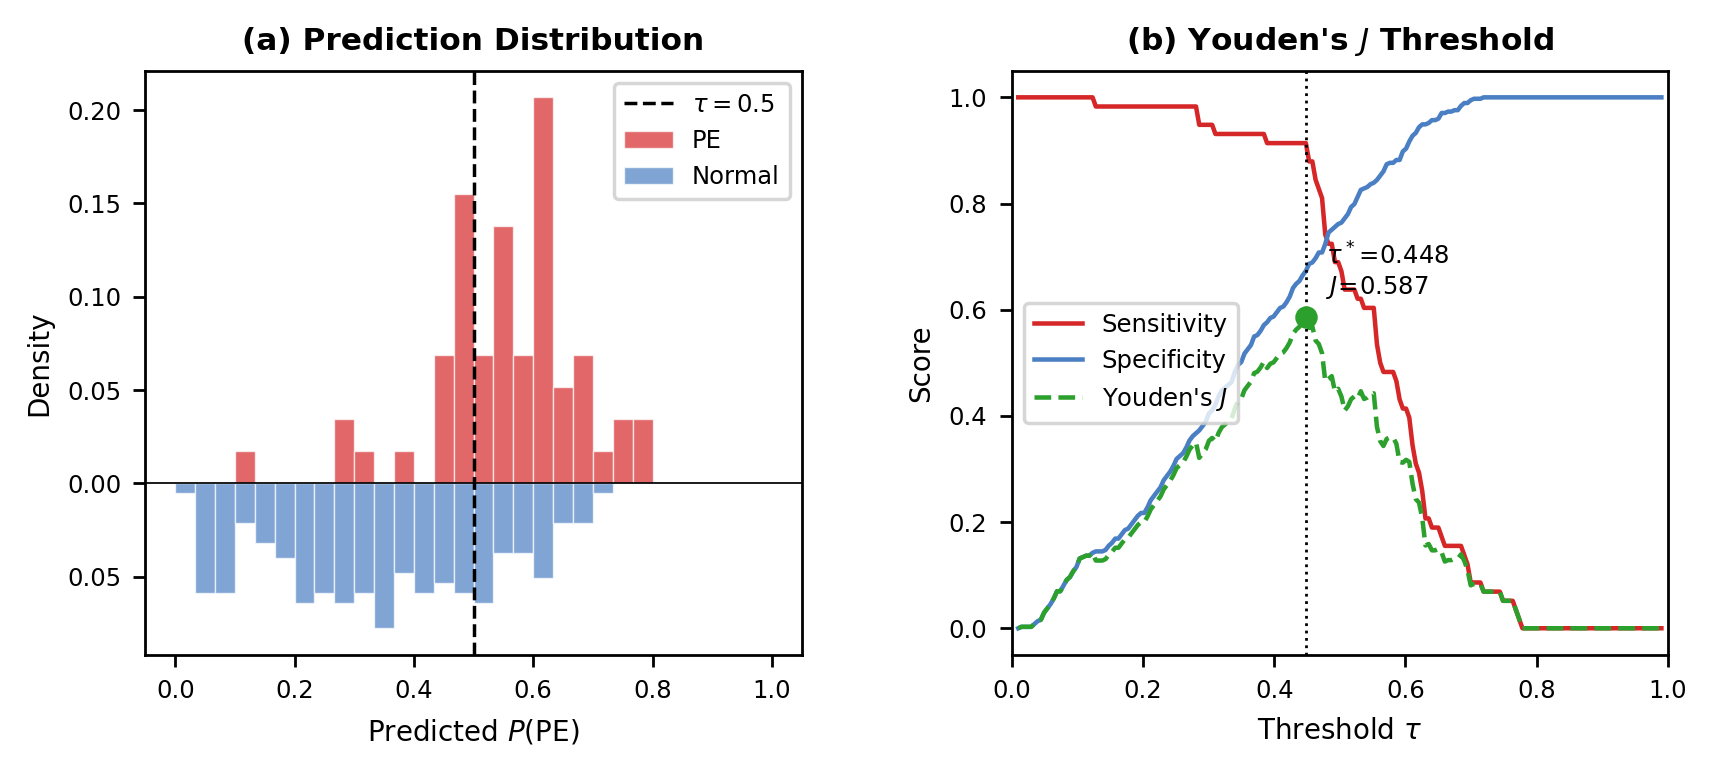
\includegraphics[width=\columnwidth]{fig_pred_youden.png}
\caption{(a) Mirror histogram of predicted $P(\text{PE})$ by true class. (b) Threshold sweep: sensitivity, specificity, and Youden's $J$. Optimal $\tau^*{=}0.448$ maximizes $J{=}0.587$.}
\label{fig:pred_youden}
\end{figure}

\section{Random Forest Featurization Progress}
Decision tree-based models have proven to be successful in predicting preeclampsia, though none through the use of ECGs for inference.
\subsection{Previous Work}

 Bulez et al observed the use of a LightGBM model using data from blood tests, blood pressure, and other factors from patient EHRs with the conclusion that age and features from the blood test were most important for inference . In Zhang et al's work, the XGBoost model was used on urine samples to determine seven compounds that were most important in predicting preeclampsia .

\subsection{Evaluation Criteria}

As a binary classification problem, the main metrics used in determining the model performance will be area under curve (AUC), accuracy, precision, recall, and F1-score. MUSE values of certain features are reported from the UCDH Echo dataset which will be compared to features created locally from Neurokit to determine accurate implementation. Once the featurizations have been implemented, feature importance analysis will be used to determine which features from the ECGs are most useful for prediction, ultimately pruning the features by analyzing trade-offs from the performance metrics.

\subsection{Implementation and Results}

The Python library Neurokit has methods for cleaning ECG signals along with extracting certain features. Through the use of these methods, we are able to implement the features in Table~\ref{tab:ecg-features}. Hana Shaik, our graduate mentor, has already implemented ST-T abnormalities and used these features in detecting RWMA. Testing occurred on the Nightingale ECG dataset to ensure that featurization was occurring. As another form of validation, we were able to compare our implementation to Hana's implementation. After receiving the balanced UCDH Echo dataset, we reformatted our Nightingale code to be able to process individual CSV ECG files instead of individual lead files. We had to drop three ECGs due to zeros in some leads or NaNs after delineation.

The main issue as of the moment is figuring out accurate QRS axis and T-axis calculations in order to also obtain the frontal QRS-T angle. Currently we have two implementations for the QRS axis. The first is the isoelectric method, which estimates the axis by pinpointing the isoelectric lead and going $\pm 90^{\circ}$ based on whether the perpendicular pair has a positive or negative QRS value. The second uses the equation $\text{QRS-axis} = \pm \arctan\!\left(\frac{2 \cdot \text{aVF}}{\sqrt{3} \cdot \text{I}}\right)$, which gives a specific numeric value, though in clinical practice small degree differences are insignificant .

\begin{table}[H]
\centering
\caption{ECG Features and Their Equations}
\label{tab:ecg-features}
\setlength{\arrayrulewidth}{0.4pt}
\renewcommand{\arraystretch}{1.25}
\begin{tabular}{@{}ll@{}}
\toprule
\textbf{Feature} & \textbf{Equation} \\
\toprule
\multicolumn{2}{@{}l@{}}{\textit{\textbf{P-Wave Features}}} \\[2pt]
$P_{\max}$ & $\max_{\ell \in \mathcal{L}}(P_{\text{off}}^{\ell} - P_{\text{on}}^{\ell})$ \\
$P_{\min}$ & $\min_{\ell \in \mathcal{L}}(P_{\text{off}}^{\ell} - P_{\text{on}}^{\ell})$ \\
P-Wave Dispersion & $P_{\max} - P_{\min}$ \\
\specialrule{1.2pt}{2pt}{2pt}
\multicolumn{2}{@{}l@{}}{\textit{\textbf{QT Features}}} \\[2pt]
QT Dispersion & $QT_{\max} = \max_{\ell \in \mathcal{L}}(T_{\text{off}}^{\ell} - R_{\text{on}}^{\ell})$ \\
 & $QT_{\min} = \min_{\ell \in \mathcal{L}}(T_{\text{off}}^{\ell} - R_{\text{on}}^{\ell})$ \\
 & $QT_{\max} - QT_{\min}$ \\
$T_{pe}$ Interval & $\text{mean}(T_{\text{off}} - T_{\text{peak}})$ \\
$T_{pe}$/QT & $T_{pe}\text{ Interval} \;/\; \text{mean}(T_{\text{off}} - R_{\text{on}})$ \\
$T_{pe}$/QTc & $(T_{pe}/\text{QT}) \;/\; \sqrt{\text{mean}(\Delta R_{\text{peak}})}$ \\
\specialrule{1.2pt}{2pt}{2pt}
\multicolumn{2}{@{}l@{}}{\textit{\textbf{ST Features}}} \\[2pt]
ST Elevation & $\mathbf{1}$ if $>50\%$ elevated,\ $\mathbf{0}$ otherwise \\
ST Depression & $\mathbf{1}$ if $>50\%$ depressed,\ $\mathbf{0}$ otherwise \\
Avg.\ Amp.\ Diff. & $\text{mean}(A_{\text{ST}} - A_{\text{PR}})$ \\
Med.\ Amp.\ Diff. & $\text{med}(A_{\text{ST}} - A_{\text{PR}})$ \\
Max.\ Amp.\ Diff. & $\max(A_{\text{ST}} - A_{\text{PR}})$ \\
Min.\ Amp.\ Diff. & $\min(A_{\text{ST}} - A_{\text{PR}})$ \\
\specialrule{1.2pt}{2pt}{2pt}
\multicolumn{2}{@{}l@{}}{\textit{\textbf{Axis Features}}} \\[2pt]
QRS Axis & TBD \\
T Axis & TBD \\
Frontal QRS-T Angle & $|\,\text{QRS Axis} - \text{T Axis}\,|$ \\
\bottomrule
\end{tabular}
\end{table}

\subsection{Future Work}

With the UCDH Echo dataset and MUSE values now released, we will be able to compare Neurokit values to MUSE values and determine if there are any drastic differences. One issue is there is not a reported value for the QRS axis nor a specific equation the MUSE developers used, so we will have to experiment through feature analysis to determine if our implementations are important for inference. An RF model will be initially used, but other decision tree models will be tested such as LightGBM and XGBoost to achieve best performance. After model selection, feature importance and feature distribution will be analyzed through $\chi^2$ testing or principal component analysis (PCA). Because the dataset is imbalanced, we may employ SMOTE to train on a balanced dataset.

\newpage
\section{Convolutional Transformer Progress}

In this report we cover the process of arriving at our baseline model, enhancements we have made thus far, as well as directions we plan to take for the three weeks until Progress Report 2 where we intend to have a fully functional model and report for submission to Sandia, and use the remainder of the time to prepare our live presentation and showcase demonstration.

We performed exploratory data analysis to inform our initial model architecture to perform both narrow studies modifying parameters with Optuna, and broad studies modifying architecture to see what sticks.

\subsection{Previous Work}

We build off of the work by Butler et al.\ and their ECG-AI which we have obtained from GitHub . ECG-AI is a ResNet-based 1-D CNN that accepts 12-lead ECG signals of length 2250 samples as a channel-dependent input. The architecture comprises six residual blocks organized into three stages of progressively increasing filter width (16, 32, 64). All convolutions use kernel size 3 with L2 regularization ($\lambda = 10^{-4}$). Each block ends with max-pooling and dropout (0.1). Blocks 3 and 5 (the first block of Stages 2 and 3) additionally use strided convolutions (stride=2) with a $1\times1$ projection for the skip connection to match the increased filter count. A final flatten and dense softmax layer produces a two-class output.

\begin{figure}[H]
\centering
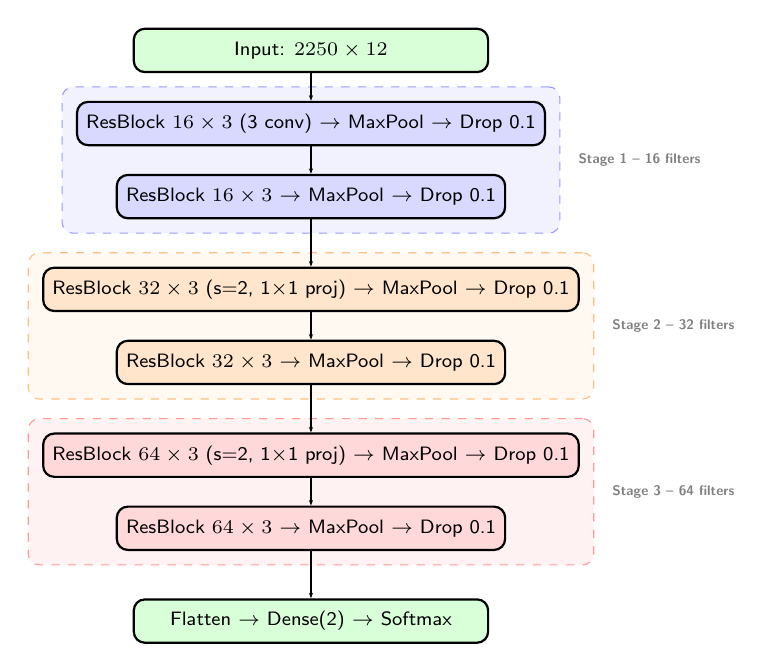
\begin{tikzpicture}[
    node distance=0.35cm,
    block/.style={draw, rounded corners, minimum height=0.55cm, minimum width=4.5cm,
                  font=\scriptsize\sffamily, align=center, thick},
    stage16/.style={block, fill=blue!15},
    stage32/.style={block, fill=orange!20},
    stage64/.style={block, fill=red!15},
    io/.style={block, fill=green!15},
    arrow/.style={-{Stealth[length=2pt]}, thick},
    stagelabel/.style={font=\tiny\sffamily\bfseries, text=gray},
]

\node[io] (input) {Input: $2250\times12$};
\node[stage16, below=of input] (rb1) {ResBlock $16\times3$ (3 conv) $\to$ MaxPool $\to$ Drop 0.1};
\node[stage16, below=of rb1] (rb2) {ResBlock $16\times3$ $\to$ MaxPool $\to$ Drop 0.1};
\node[stage32, below=0.6cm of rb2] (rb3) {ResBlock $32\times3$ (s=2, 1$\times$1 proj) $\to$ MaxPool $\to$ Drop 0.1};
\node[stage32, below=of rb3] (rb4) {ResBlock $32\times3$ $\to$ MaxPool $\to$ Drop 0.1};
\node[stage64, below=0.6cm of rb4] (rb5) {ResBlock $64\times3$ (s=2, 1$\times$1 proj) $\to$ MaxPool $\to$ Drop 0.1};
\node[stage64, below=of rb5] (rb6) {ResBlock $64\times3$ $\to$ MaxPool $\to$ Drop 0.1};
\node[io, below=0.6cm of rb6] (flat) {Flatten $\to$ Dense(2) $\to$ Softmax};

\foreach \a/\b in {input/rb1, rb1/rb2, rb2/rb3, rb3/rb4, rb4/rb5, rb5/rb6, rb6/flat}{
    \draw[arrow] (\a) -- (\b);
}

\begin{scope}[on background layer]
    \node[fit=(rb1)(rb2), inner sep=5pt, draw=blue!40, fill=blue!5, rounded corners, dashed] (s1) {};
    \node[stagelabel, right=3pt of s1] {Stage 1 -- 16 filters};
    \node[fit=(rb3)(rb4), inner sep=5pt, draw=orange!50, fill=orange!5, rounded corners, dashed] (s2) {};
    \node[stagelabel, right=3pt of s2] {Stage 2 -- 32 filters};
    \node[fit=(rb5)(rb6), inner sep=5pt, draw=red!40, fill=red!5, rounded corners, dashed] (s3) {};
    \node[stagelabel, right=3pt of s3] {Stage 3 -- 64 filters};
\end{scope}

\end{tikzpicture}
\caption{High-level view of the Butler et al.\ ECG-AI architecture showing six ResBlocks across three filter-width stages (16, 32, 64). Block~1 contains three convolutions; Blocks~3 and~5 use strided convolutions (s=2) with $1\times1$ projections for dimensionality matching. All blocks end with max-pooling and dropout.}
\label{fig:butler-arch}
\end{figure}

The progressively increasing filter width means more feature interpretations at earlier layers as the receptive field grows. We begin with simple patterns which might just be some sort of sequences of values, but their successive compositions begin to capture clinical features . We will also utilize the architecture of successively increasing ResNet blocks for our baseline model.

\subsection{Channel Independence via Lead Correlation}

To determine whether the 12 ECG leads should be processed jointly (channel-dependent) or independently (channel-independent), we measure how much preeclampsia disrupts the inter-lead correlation structure. For each recording $n$, we compute the $12 \times 12$ Pearson correlation matrix $C^{(n)}$ across leads, then average within each class

\begin{equation}
\bar{C}_{\text{PE}} = \frac{1}{N_{\text{PE}}} \sum_{n \in \text{PE}} C^{(n)}, \qquad
\bar{C}_{\text{Normal}} = \frac{1}{N_{\text{Normal}}} \sum_{n \in \text{Normal}} C^{(n)}
\end{equation}

We then compute the Frobenius norm of the difference:

\begin{equation}
\| \bar{C}_{\text{PE}} - \bar{C}_{\text{Normal}} \|_F = \sqrt{\sum_{i=1}^{12}\sum_{j=1}^{12} \left(\bar{C}_{\text{PE},ij} - \bar{C}_{\text{Normal},ij}\right)^2} = 1.026
\end{equation}

A high Frobenius norm ($>2.0$) would indicate that preeclampsia significantly alters how leads correlate with each other, meaning the cross-lead relationship itself is a discriminative feature best captured by 2D convolution across leads. Our value of 1.026 indicates only modest disruption --- the leads correlate roughly the same way in both classes. The discriminative information therefore resides within each lead's waveform, not in inter-lead coupling, justifying per-lead 1D convolution (channel-independent processing).

ECG-AI inputs the entire $12 \times 2250$ data matrix into the CNN, where all leads mix from the first convolutional layer. RepNet instead processes each lead through its own 1D CNN stream, extracting per-lead features before combining them via cross-lead attention in subsequent stages.

\begin{figure}[H]
\centering
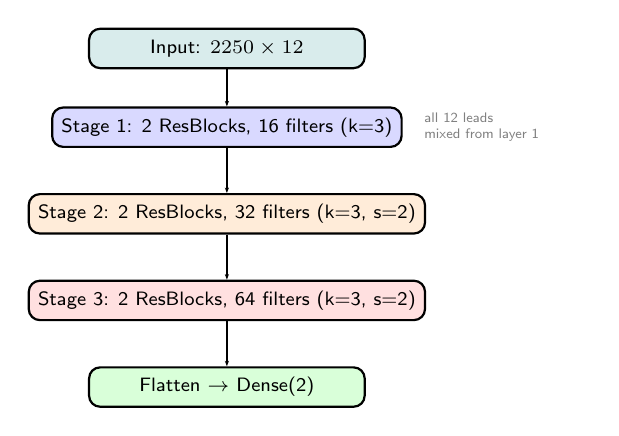
\begin{tikzpicture}[
    node distance=0.35cm,
    box/.style={draw, rounded corners, minimum height=0.5cm, font=\scriptsize\sffamily, align=center, thick},
    lead/.style={box, fill=teal!15},
    conv/.style={box, fill=blue!15},
    outnode/.style={box, fill=green!15},
    arrow/.style={-{Stealth[length=2pt]}, thick},
    lbl/.style={font=\tiny\sffamily, text=gray},
]

\node[lead, minimum width=3.5cm] (input_b) at (0, 0) {Input: $2250\times12$};
\node[conv, minimum width=3.5cm] (conv_b) at (0, -1) {Stage 1: 2 ResBlocks, 16 filters (k=3)};
\node[conv, minimum width=3.5cm, fill=orange!15] (res_b) at (0, -2.1) {Stage 2: 2 ResBlocks, 32 filters (k=3, s=2)};
\node[conv, minimum width=3.5cm, fill=red!12] (res_c) at (0, -3.2) {Stage 3: 2 ResBlocks, 64 filters (k=3, s=2)};
\node[outnode, minimum width=3.5cm] (out_b) at (0, -4.3) {Flatten $\to$ Dense(2)};

\draw[arrow] (input_b) -- (conv_b);
\draw[arrow] (conv_b) -- (res_b);
\draw[arrow] (res_b) -- (res_c);
\draw[arrow] (res_c) -- (out_b);

\node[lbl, right=0.15cm of conv_b, text width=2cm] {all 12 leads\\mixed from layer 1};

\end{tikzpicture}
\caption{ECG-AI channel-dependent input. All 12 leads are fed as channels into a shared CNN, where leads mix from the first convolutional layer.}
\label{fig:butler-channel-dep}
\end{figure}

\begin{figure}[H]
\centering
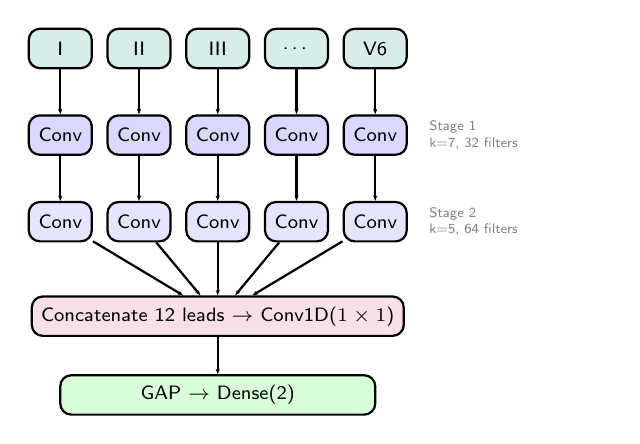
\begin{tikzpicture}[
    node distance=0.35cm,
    box/.style={draw, rounded corners, minimum height=0.5cm, font=\scriptsize\sffamily, align=center, thick},
    lead/.style={box, fill=teal!15, minimum width=0.8cm},
    conv/.style={box, fill=blue!15, minimum width=0.8cm},
    fuse/.style={box, fill=purple!12, minimum width=4cm},
    outnode/.style={box, fill=green!15, minimum width=4cm},
    arrow/.style={-{Stealth[length=2pt]}, thick},
    lbl/.style={font=\tiny\sffamily, text=gray},
]

% Individual lead inputs
\foreach \i/\lead in {0/I, 1/II, 2/III, 3/\dots, 4/V6} {
    \pgfmathsetmacro{\xpos}{-2 + \i * 1.0}
    \node[lead] (in_\i) at (\xpos, 0) {\lead};
}

% Stage 1: per-lead conv
\foreach \i in {0,1,2,3,4} {
    \pgfmathsetmacro{\xpos}{-2 + \i * 1.0}
    \node[conv] (s1_\i) at (\xpos, -1.1) {Conv};
    \draw[arrow] (in_\i) -- (s1_\i);
}
\node[lbl, right=0.15cm of s1_4, text width=2.2cm] {Stage 1\\k=7, 32 filters};

% Stage 2: per-lead conv
\foreach \i in {0,1,2,3,4} {
    \pgfmathsetmacro{\xpos}{-2 + \i * 1.0}
    \node[conv, fill=blue!10] (s2_\i) at (\xpos, -2.2) {Conv};
    \draw[arrow] (s1_\i) -- (s2_\i);
}
\node[lbl, right=0.15cm of s2_4, text width=2.2cm] {Stage 2\\k=5, 64 filters};

% Fusion
\node[fuse] (fuse) at (0, -3.4) {Concatenate 12 leads $\to$ Conv1D($1\times1$)};
\foreach \i in {0,1,2,3,4} {
    \draw[arrow] (s2_\i) -- (fuse);
}

\node[outnode] (out_r) at (0, -4.4) {GAP $\to$ Dense(2)};
\draw[arrow] (fuse) -- (out_r);

\end{tikzpicture}
\caption{RepNet Baseline architecture. Each lead is processed through independent Conv1D streams across two stages with no cross-lead interaction until fusion. GAP collapses the full temporal dimension, providing full-sequence context despite the small convolutional receptive field of 32 samples.}
\label{fig:repnet-baseline-arch}
\end{figure}

\subsection{Kernel Size / Layer Depth for Receptive Field}
Power spectral density (PSD) decomposes a signal into its frequency components and reveals where the energy is concentrated. For each lead $\ell$ and recording $n$, PSD is estimated via Welch's method, which divides the signal $x^{(n)}_\ell(t)$ into overlapping segments, windows each with a Hann function, computes the periodogram of each segment, and averages them .

\begin{equation}
\hat{S}^{(n)}_\ell(f) = \frac{1}{K} \sum_{k=1}^{K} \left| \text{DFT}\left[ w(t) \cdot x^{(n)}_{\ell,k}(t) \right] \right|^2
\end{equation}

\noindent where $K$ is the number of segments, $w(t)$ is the window function, and $x^{(n)}_{\ell,k}(t)$ is the $k$-th segment. Averaging across all recordings within each class yields class-level PSD estimates $\bar{S}_{\text{PE}}(f)$ and $\bar{S}_{\text{Normal}}(f)$. The frequency $f_{\text{peak}}$ at which their absolute difference is maximized indicates where the discriminative signal lives. At 250\,Hz sampling with a segment length of 512 samples, this yields a frequency resolution of approximately 0.49\,Hz.

See Appendix~\ref{appendix:psd} for the full per-lead PSD comparison. The greatest class divergence occurs at approximately 1\,Hz across all leads, indicating that the discriminative signal is concentrated at low frequencies.

To capture a feature at frequency $f$, a convolutional receptive field must span at least one full cycle of that frequency. At 250\,Hz, one cycle of the 1\,Hz discriminative peak corresponds to 250 samples. A network's receptive field must therefore exceed 250 samples for the convolutional pathway alone to detect this feature. Rather than using a single large kernel, smaller convolutions are stacked with max-pooling, where each pooling layer doubles the effective stride and the receptive field grows geometrically with depth. The receptive field at layer $l$ follows:

\begin{equation}
\text{RF}_l = \text{RF}_{l-1} + (k_l - 1) \times \prod_{j=1}^{l-1} s_j
\end{equation}

\noindent where $k_l$ is the kernel size and $s_j$ is the stride (including pooling) at layer $j$. Tables~\ref{tab:rf-ecgai} and~\ref{tab:rf-repnet} compare the receptive field buildup between ECG-AI and RepNet Baseline.

\begin{table}[H]
\centering
\caption{ECG-AI receptive field buildup. Six blocks with k=3 and strided convolutions at stage transitions (Blocks 3, 5).}
\label{tab:rf-ecgai}
\small
\begin{tabular}{lr}
\toprule
\textbf{Layer} & \textbf{RF (samples)} \\
\midrule
Input & 1 \\
Block 1: 3$\times$Conv(k=3) + Pool & 8 \\
Block 2: 2$\times$Conv(k=3) + Pool & 18 \\
Block 3: 2$\times$Conv(k=3, s=2) + Proj + Pool & 38 \\
Block 4: 2$\times$Conv(k=3) + Pool & 78 \\
Block 5: 2$\times$Conv(k=3, s=2) + Proj + Pool & 158 \\
Block 6: 2$\times$Conv(k=3) + Pool & 318 \\
\midrule
\textbf{Final RF} & \textbf{318 (1.27\,s)} \\
\bottomrule
\end{tabular}
\end{table}

ECG-AI reaches a receptive field of 318 samples (1.27\,s) through six blocks of small k=3 kernels with strided convolutions at stage transitions, comfortably exceeding the 250-sample threshold. RepNet Baseline reaches only 32 samples (0.13\,s) with two blocks --- far short of the 250-sample target for capturing the 1\,Hz discriminative feature. However, the global average pooling (GAP) at the fusion stage collapses the entire remaining temporal dimension, giving the classifier access to information across the full 2500-sample (10\,s) input.


\begin{table}[H]
\centering
\caption{RepNet Baseline receptive field buildup. Two blocks with wider kernels (k=7, k=5), each containing two convolutions followed by max-pooling.}
\label{tab:rf-repnet}
\small
\begin{tabular}{lr}
\toprule
\textbf{Layer} & \textbf{RF (samples)} \\
\midrule
Input & 1 \\
Stage 1: 2$\times$Conv(k=7) + Pool & 14 \\
Stage 2: 2$\times$Conv(k=5) + Pool & 32 \\
\midrule
\textbf{Final conv RF} & \textbf{32 (0.13\,s)} \\
\bottomrule
\end{tabular}
\end{table}

We note that the RepNet Baseline and Hybrid architectures were created before this exploratory data analysis and architectural deconstruction of ECG-AI were performed. The current two-stage designs with a 32-sample receptive field do not yet reflect the 250-sample target derived from the PSD analysis. However, we have some training history and performance baselines on them that we want to use to inform incremental scaling rather than naively copying larger architectures.

\subsection{Experimenting with Cross-Lead Attention}

We inserted cross-lead multi-head self-attention blocks between the baseline convolutional stages to explore whether allowing leads to interact before fusion would improve classification. The attention mechanism pools each lead's feature map to a single token, applies self-attention across the 12 lead tokens, and gates each lead's full feature map with the resulting weights.

\begin{figure}[H]
\centering
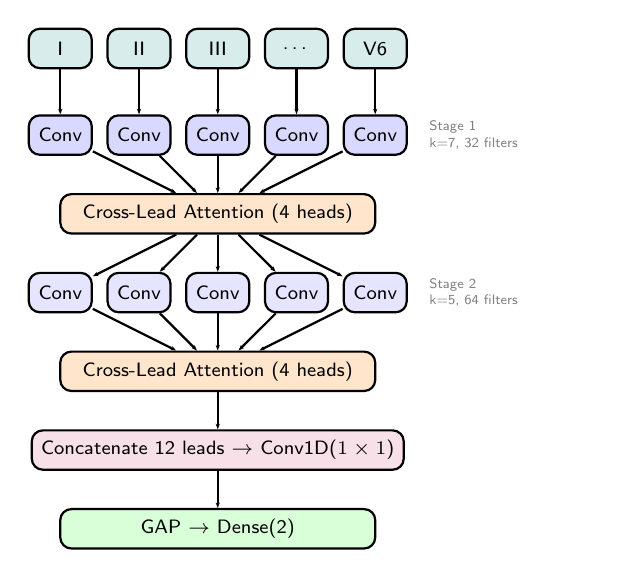
\begin{tikzpicture}[
    node distance=0.35cm,
    box/.style={draw, rounded corners, minimum height=0.5cm, font=\scriptsize\sffamily, align=center, thick},
    lead/.style={box, fill=teal!15, minimum width=0.8cm},
    conv/.style={box, fill=blue!15, minimum width=0.8cm},
    attn/.style={box, fill=orange!20, minimum width=4cm},
    fuse/.style={box, fill=purple!12, minimum width=4cm},
    outnode/.style={box, fill=green!15, minimum width=4cm},
    arrow/.style={-{Stealth[length=2pt]}, thick},
    lbl/.style={font=\tiny\sffamily, text=gray},
]

% Individual lead inputs
\foreach \i/\lead in {0/I, 1/II, 2/III, 3/\dots, 4/V6} {
    \pgfmathsetmacro{\xpos}{-2 + \i * 1.0}
    \node[lead] (in_\i) at (\xpos, 0) {\lead};
}

% Stage 1: per-lead conv
\foreach \i in {0,1,2,3,4} {
    \pgfmathsetmacro{\xpos}{-2 + \i * 1.0}
    \node[conv] (s1_\i) at (\xpos, -1.1) {Conv};
    \draw[arrow] (in_\i) -- (s1_\i);
}
\node[lbl, right=0.15cm of s1_4, text width=2.2cm] {Stage 1\\k=7, 32 filters};

% Cross-lead attention 1
\node[attn] (attn1) at (0, -2.1) {Cross-Lead Attention (4 heads)};
\foreach \i in {0,1,2,3,4} {
    \draw[arrow] (s1_\i) -- (attn1);
}

% Stage 2: per-lead conv
\foreach \i in {0,1,2,3,4} {
    \pgfmathsetmacro{\xpos}{-2 + \i * 1.0}
    \node[conv, fill=blue!10] (s2_\i) at (\xpos, -3.1) {Conv};
}
\draw[arrow] (attn1) -- (s2_0);
\draw[arrow] (attn1) -- (s2_1);
\draw[arrow] (attn1) -- (s2_2);
\draw[arrow] (attn1) -- (s2_3);
\draw[arrow] (attn1) -- (s2_4);
\node[lbl, right=0.15cm of s2_4, text width=2.2cm] {Stage 2\\k=5, 64 filters};

% Cross-lead attention 2
\node[attn] (attn2) at (0, -4.1) {Cross-Lead Attention (4 heads)};
\foreach \i in {0,1,2,3,4} {
    \draw[arrow] (s2_\i) -- (attn2);
}

% Fusion
\node[fuse] (fuse) at (0, -5.1) {Concatenate 12 leads $\to$ Conv1D($1\times1$)};
\draw[arrow] (attn2) -- (fuse);

\node[outnode] (out_r) at (0, -6.1) {GAP $\to$ Dense(2)};
\draw[arrow] (fuse) -- (out_r);

\end{tikzpicture}
\caption{RepNet Hybrid architecture. Per-lead Conv1D streams are interleaved with cross-lead multi-head self-attention, allowing leads to dynamically weight each other after each convolutional stage.}
\label{fig:repnet-hybrid-arch}
\end{figure}

 Initial experiments indicated a slight increase in performance over the baseline, so we then performed a broad Optuna hyperparameter study optimizing learning rate and dropout rate over 20 trials that took a few hours to complete overnight. This gives us an estimate for the combinatorial explosion of larger training jobs, and how we should allocate our time and compute resources accordingly.

\begin{table}[H]
\centering
\caption{RepNet Hybrid Optuna best trial results (Trial \#12 of 20).}
\label{tab:optuna-results}
\small
\begin{tabular}{lr}
\toprule
\multicolumn{2}{l}{\textbf{Best Hyperparameters}} \\
\midrule
Learning rate & $8.76 \times 10^{-4}$ \\
Dropout & 0.064 \\
CV AUROC (5-fold) & 0.8018 \\
Test AUROC & 0.7873 \\
\bottomrule
\end{tabular}

\vspace{0.5em}
\begin{tabular}{lrr}
\toprule
& \textbf{$t = 0.50$} & \textbf{Youden's $J = 0.786$} \\
\midrule
Accuracy & 0.73 & 0.76 \\
PE Precision & 0.70 & 0.76 \\
PE Recall & 0.84 & 0.76 \\
PE F1-score & 0.76 & 0.76 \\
Normal Precision & 0.79 & 0.75 \\
Normal Recall & 0.61 & 0.75 \\
Normal F1-score & 0.69 & 0.75 \\
\bottomrule
\end{tabular}
\end{table}

The below contour plot shows that the model benefits from lower learning rates when dropout is also low. This contradicts empirical results from papers suggesting higher dropout rates to prevent overfitting, so more work is needed to understand this interaction.




\subsection{Discussion}
All above analysis and model architecture discovery was performed on a pre-balanced subset of the UC Davis Health preeclampsia dataset. Near completing this report we have received the full unbalanced dataset, which will inform more aggressive architectural scaling, fine-tuning, and exploration of augmentation and synthetic data generation.

\begin{table}[H]
\centering
\caption{UC Davis Health preeclampsia dataset distribution.}
\label{tab:ucdh-dataset}
\small
\begin{tabular}{lrr}
\toprule
& \textbf{Balanced} & \textbf{Full} \\
\midrule
Normal patients & 132 & 1,217 \\
Normal ECGs & 182 & 1,854 \\
\midrule
PE patients & 132 & 132 \\
PE ECGs & 187 & 187 \\
\midrule
\textbf{Total ECGs} & \textbf{369} & \textbf{2,041} \\
Ratio (Normal:PE) & $\sim$1:1 & $\sim$9.9:1 \\
\bottomrule
\end{tabular}
\end{table}

\subsection{Future Work}

We will experiment with a vast variety of experimental architectures from literature and creative ideas looking at the data, model performance, layer behavior, and Optuna feedback. We will have to determine what is to be done about the severe class imbalance of the full dataset, we will most likely experiment with SMOTE-Tomek , a synthetic minority oversampling technique combined with Tomek link cleaning, and we will experiment with GAN models built for synthetic generation of ECG data .

We will analyze dimensionality reduction of our inputs, determining which leads are relevant for diagnosis of preeclampsia. Dimensionality reduction is relevant because a fully-kitted 12-lead ECG is still a less common measure used in larger clinics and hospitals. In any situation such as for paramedics, smaller clinics, or even the developing world where preeclampsia disproportionately kills, it would be useful to still be able to draw conclusions even with constrained diagnostic resources. Such would enable using simpler non 12-lead ECG systems, and diagnosis from local and embedded compute on the spot rather than needing external compute clusters on premises or in the cloud.

We will perform dimensionality reduction using principal component analysis (PCA) on both waveforms and features to determine the data with the most variance that may contribute most to classification, and experiment with models set only to have inputs from them, and furthermore only to train on them.

We will also do ablation studies, where we selectively add or remove information such as masking certain leads, or injecting noise, to see what actually breaks the model versus leaves it unchanged. At the extreme we can do a combinatorial study of every possible subset of the 12-lead ECG, 2 to the power of 12 being 4096 sets, if compute constraints are not an issue such as cloud computing .

Lastly we may train an autoencoder such as BERT across leads to learn a compressed latent representation, and by varying bottleneck size we can see performance vs information capacity, seeing how much information we can compress and still retain performance, showing us how much information we can discard or start with in the first place. This would essentially be a continuous version of channel dropout mentioned earlier.


\section{Caliper Libtorch Visualization Utility}
The development of our model will ship alongside Caliper, a framework built atop of C++, Libtorch (Pytorch C++ API), and OpenGL, ImGui and ImPlot. It is publicly available through GitHub. It is a highly performant machine learning visualization tool able to display data elements, neural network layers, outputs in real time, and tie them to arbitrary rendering through whatever is possible with a 3D graphics API, and also offering a user interface to alter settings on the fly.

Development of the basic framework has been successful, with CUDA augmentation on Windows and MPS augmentation on macOS. We have created a small applet to play around with baseline wander high pass filter in real time, and scrub the entire dataset instantaneously without delay.  We are planning to have options to load ECG datasets in the format of CSV and then options to load models from standard PyTorch weight formats that can then automatically construct visualizations that can also show data propagation through the network.

For this research project specifically, we will have ECG waveforms be displayed and show the translation of convolutional kernels and the attention map highlighting regions of interest for classification, and alongside that have the random forest classifier and its extraction of manual features be indicated so that there is explainability for the classification. We can showcase that a clinician can point to a heatmap and also state that a certain heartbeat feature has deviated from a healthy range.

Though Caliper can implement training, it is not intended for this project as our workflow needs to be universally deployable in Python, with libraries that are not available in C++. But for much more intensive and performant projects Caliper could be utilized. We intend to use Caliper to demonstrate our model's features at our tabling in the Davis Senior Design Showcase in June 2026, providing attendees with an opportunity to interact with our research.

\section{Conclusion}
We have completed a comprehensive review of the literature spanning preeclampsia ML, ECG classification, transformer architectures, foundation models, data augmentation, and model efficiency. We have identified that ECG waveform classification for preeclampsia is a largely untapped field with only one prior deep learning study. From those insights we have created a baseline for our own novel architecture and intend to further expand and experiment with the architecture to refine it. On the random forest side, we have implemented ECG featurization using Neurokit2 and validated our implementation against existing work. Data augmentation via SMOTE or transformer GAN will be explored to address class imbalance. Development of the Caliper visualization utility will continue in parallel to provide real time explainability for our models at the Davis Senior Design Showcase in June 2026.

As we continue our model architecting and optimizing studies, we will conduct ablation studies and dimensionality reduction experiments to determine the minimum lead configuration necessary for performant classification. An important aspect of this project is building pipelines and systems that can run autonomously on our most powerful compute so we can dedicate time to other aspects of the project.

\appendix
\clearpage
\onecolumn
\section{Summary of Reviewed Literature}
\label{appendix:literature}

\begin{table*}[h]
\caption{Summary of Reviewed Literature}
\label{tab:literature}
\small
\centering
\begin{tabular}{cp{0.26\textwidth}p{0.12\textwidth}p{0.44\textwidth}}
\toprule
\textbf{Read} & \textbf{Paper} & \textbf{Type} & \textbf{Purpose} \\
\midrule
\multicolumn{4}{l}{\textbf{Phase 1 --- Exploratory Review}} \\[2pt]
\multicolumn{4}{l}{\textit{Preeclampsia ML Literature Reviews}} \\
$\checkmark$ & Özcan et al.~ & Review & General overview of ML models in preeclampsia \\
 & Liu et al.~ & Review & Statistical meta-analysis of ML models in preeclampsia \\
\midrule
\multicolumn{4}{l}{\textit{Preeclampsia ECG Classification Studies}} \\
$\checkmark$ & Butler et al.~ & Original & 1-D CNN for preeclampsia ECG classification \\
$\checkmark$ & Euliano et al.~ & Original & ECG and photoplethysmography features for preeclampsia diagnosis \\
\midrule
\multicolumn{4}{l}{\textit{ECG Classification Machine Learning}} \\
$\checkmark$ & Boulif et al.~ & Review & Broad overview of ECG classification methods \\
 & Prakash et al.~ & Review & Systematic review of ML and DL for ECG beat classification \\
\midrule
\multicolumn{4}{l}{\textit{ECG Classification DL Literature Reviews}} \\
$\checkmark$ & Y. Ansari et al.~ & Review & Overview of DL architectures for ECG (2017-2023) \\
$\checkmark$ & M. Ansari et al.~ & Review & Survey of transformers and LLMs for ECG processing \\
\midrule
\multicolumn{4}{l}{\textit{Capstone Project Assigned Literature}} \\
$\checkmark$ & Butler et al.~ & Original & 1-D CNN for preeclampsia ECG classification \\
$\checkmark$ & Joshi et al.~ & Original & RF and CNN bicameral approach for ECG waveform classification \\
$\checkmark$ & Xue et al.~ & Original & DL interpretation from reduced ECG lead sets vs.\ full 12-lead \\
$\checkmark$ & Attia et al.~ & Original & AI detection of low ejection fraction from a single-lead ECG \\
\midrule
\multicolumn{4}{l}{\textit{Random Forest Featurization Progress}} \\
$\checkmark$ & Bulez et al.~ & Original & LightGBM on EHR data for early preeclampsia diagnosis \\
$\checkmark$ & Zhang et al.~ & Original & XGBoost on urine metabolomics for preeclampsia prediction \\
$\checkmark$ & Scherer et al.~ & Original & T-wave axis association with coronary artery calcification \\
\midrule
\multicolumn{4}{l}{\textbf{Phase 2 --- Enhancement Review}} \\[2pt]
\multicolumn{4}{l}{\textit{ECG Waveform Preprocessing Reviews}} \\
 & Jia et al.~ & Review & Overview of ECG preprocessing techniques \\
 & Satija et al.~ & Review & Overview of ECG signal quality assessment techniques \\
\midrule
\multicolumn{4}{l}{\textit{Preeclampsia ECG Waveform Features}} \\
 & Angeli et al.~ & Original & Review of ECG features associated with preeclampsia \\
 & Raffaelli et al.~ & Original & QT dispersion and ventricular repolarization in preeclampsia \\
\midrule
\multicolumn{4}{l}{\textit{ECG Feature Analysis Literature Reviews}} \\
 & Kaplan et al.~ & Review & General overview of ECG feature analysis \\
 & Singh et al.~ & Review & General overview of ECG feature extraction \\
\midrule
\multicolumn{4}{l}{\textit{Data Augmentation for ECG Waveforms}} \\
 & Rahman et al.~ & Review & Overview of ECG data augmentation strategies \\
 & Xia et al.~ & Original & Transformer GAN for ECG data augmentation \\
\midrule
\multicolumn{4}{l}{\textit{Preeclampsia Decision Tree Classification}} \\
 & Park et al.~ & Original & Personalized decision tree for heartbeat type classification \\
 & Musa et al.~ & Original & Decision tree with PCA for preeclampsia detection \\
\midrule
\multicolumn{4}{l}{\textit{ECG Model Efficiency and Compression}} \\
 & Keivanimehr et al.~ & Review & Survey of TinyML and edge intelligence for ECG monitoring \\
 & Gupta et al.~ & Review & Overview of efficient architectures for ECG classification \\
\bottomrule
\end{tabular}
\end{table*}

\clearpage
% Chat log macros (breakable across pages)
\newcommand{\chatuser}[1]{%
  \begin{flushright}%
  \colorbox{gray!20}{\parbox{0.78\linewidth}{\raggedright\small\textit{#1}}}%
  \end{flushright}\medskip}
\newcommand{\chatbot}[1]{%
  \begin{tcolorbox}[colback=blue!8,colframe=blue!8,boxrule=0pt,arc=0pt,breakable,
    left=6pt,right=6pt,top=4pt,bottom=4pt]%
  \raggedright\small #1%
  \end{tcolorbox}\medskip}

\section{Power Spectral Density per Lead}
\label{appendix:psd}

\clearpage
\section{ChatGPT Literature Review Query Transcript}
\label{appendix:chatgpt}

\begin{flushleft}
The following is an excerpt of GPT\,5.4 Thinking used to survey the literature.
\end{flushleft}

\chatuser{Name the top literature reviews of preeclampsia prediction using ML and DL.}

\chatbot{The strongest review papers in this niche are these five.
\begin{enumerate}
  \item \textbf{Ranjbar et al., ``Machine learning models for predicting preeclampsia: a systematic review.''} This is the one I would put at the top. It is a formal systematic review, it focuses tightly on preeclampsia prediction, and it summarizes predictive factors plus model accuracy across the ML literature. It appeared in 2023 in \textit{BMJ Open} and is also indexed in PubMed and BMC Pregnancy and Childbirth records.
  \item \textbf{Özcan and Peker, ``Preeclampsia prediction via machine learning: a systematic literature review.''} This is one of the clearest broad syntheses of the ML prediction literature. It reviews studies from 2013 onward and points out a real weakness in the field: many papers rely on small, single-center datasets and narrow geographic coverage.
  \item \textbf{Aljameel et al., ``Prediction of Preeclampsia Using Machine Learning and Deep Learning Models: A Review.''} This is the most directly relevant paper if you specifically want both \textbf{ML and DL} in the title and scope. It reviews studies published from 2018 to 2022, explicitly discusses deep learning papers, and summarizes commonly used methods such as random forest, SVM, and ANN.
  \item \textbf{Liu et al., ``Machine Learning Prediction Models for Preeclampsia.''} This 2026 paper is the newest major evidence synthesis I found, and it is a \textbf{systematic review and meta-analysis}, which gives it extra weight. Its stated goal is to evaluate model performance and clinical application value while dealing with heterogeneity in the literature.
  \item \textbf{Hennessy et al., ``Machine learning, advanced data analysis, and a role in pregnancy care? How can we help improve preeclampsia outcomes?''} This is less of a hard-nosed evidence synthesis than the papers above, yet it is still a useful review article because it frames how ML is being used in pregnancy and preeclampsia care, and it is valuable for understanding the clinical translation problem.
\end{enumerate}
If you want the cleanest ranking by rigor and usefulness for academic work, I would order them like this: \textbf{Ranjbar 2023}, \textbf{Liu 2026}, \textbf{Özcan 2024}, \textbf{Aljameel 2023}, \textbf{Hennessy 2024}. That ranking puts systematic reviews and meta-analytic work first, then the best broad surveys, then the more narrative clinical overview.

A blunt truth about this area: there are still very few genuinely high-quality reviews focused specifically on \textbf{deep learning} for preeclampsia prediction. Most of the stronger papers are really \textbf{ML-first reviews} that include some DL studies, rather than deep-learning-centered reviews built on a large mature literature.}

\chatuser{Name the top literature reviews of ECG classification using ML and DL.}

\chatbot{The top review papers on ECG classification using machine learning and deep learning are these.
\begin{enumerate}
  \item \textbf{Xiao et al., ``Deep Learning-Based ECG Arrhythmia Classification: A Systematic Review.''} This is one of the strongest and most useful reviews in the area. It is tightly focused on ECG arrhythmia classification, reviews 368 studies, and organizes the field by databases, preprocessing, model families, evaluation setups, metrics, and code availability. That makes it one of the clearest map-of-the-field papers for DL-based ECG classification.
  \item \textbf{Ebrahimi et al., ``A review on deep learning methods for ECG arrhythmia classification.''} This is an earlier landmark survey and still one of the most cited broad reviews in the subject. It is valuable because it pulled together the early wave of deep learning work on ECG classification and helped define the common architectures and workflow patterns used afterward.
  \item \textbf{Prakash et al., ``Advances in machine and deep learning for ECG beat classification: a systematic review.''} This is one of the best choices when you specifically want both \textbf{ML and DL} in scope rather than a DL-only paper. It is a recent systematic review centered on ECG beat classification and emphasizes current trends, dataset limitations, and the need for standardized, clinically usable pipelines.
  \item \textbf{Petmezas et al., ``State-of-the-Art Deep Learning Methods on Electrocardiogram Data: Systematic Review.''} This review is broader than arrhythmia classification alone, since it covers multiple ECG clinical tasks, yet it is still one of the stronger synthesis papers for understanding how deep learning methods are used on ECG data at scale. It is useful when you want ECG classification placed inside the larger ECG-analysis landscape.
  \item \textbf{Ansari et al., ``Deep learning for ECG Arrhythmia detection and classification: an overview of progress for period 2017--2023.''} This is a substantial survey focused on arrhythmia detection and classification, with emphasis on architectures and technical trends across the modern DL period. It is especially useful for readers trying to understand how CNN, RNN, hybrid, and transformer-style approaches evolved in the literature.
\end{enumerate}
If the goal is a blunt ranking by usefulness for research, I would put them in this order: \textbf{Xiao 2023}, \textbf{Prakash 2025}, \textbf{Ebrahimi 2020}, \textbf{Petmezas 2022}, \textbf{Ansari 2023}. That ranking gives priority to reviews that are systematic, directly centered on ECG classification, and broad enough to synthesize datasets, preprocessing, architectures, and evaluation quality in one place.

A hard truth about this literature is that many papers labeled as ``ECG classification reviews'' are actually narrow arrhythmia-review papers, and many of the stronger ones are \textbf{deep-learning-heavy} rather than balanced treatments of both classical machine learning and deep learning. The Prakash 2025 review stands out precisely because it more clearly spans both ML and DL.}

\chatuser{What about ones specifically regarding transformers?}

\chatbot{For ECG classification specifically regarding transformers, the field is still thin on pure review papers. The strongest dedicated review is this one.
\begin{enumerate}
  \item \textbf{Ansari et al., ``A survey of transformers and large language models for ECG signal processing and interpretation.''} This is the clearest top pick for transformer-focused ECG review literature. It is a 2025 survey in \textit{Artificial Intelligence Review} that explicitly covers transformer architectures for ECG tasks, including diagnosis and classification, and it compares transformer and LLM approaches across categories while discussing embedding design, architectural limits, and transparency issues.
\end{enumerate}
After that, the best papers are broader ECG review articles that include transformer-based classification as a substantial part of the map rather than the sole focus.
\begin{enumerate}
\setcounter{enumi}{1}
  \item \textbf{Gupta et al., ``A comprehensive review on efficient artificial intelligence approaches for electrocardiogram-based cardiac rhythm classification.''} This 2024 review is one of the better broad syntheses for rhythm classification, and it explicitly discusses current state-of-the-art AI models plus upcoming modeling methods relevant to real-time deployment. It is useful for transformer work because it places transformer-style methods inside the practical ECG classification pipeline rather than treating them as isolated model novelties.
  \item \textbf{Xiao et al., ``Deep Learning-Based ECG Arrhythmia Classification: A Systematic Review.''} This is still one of the strongest overall ECG-classification reviews. Its main value for transformer-focused reading is that it gives a rigorous systematic framework for datasets, preprocessing, task setups, metrics, and model families, which lets you situate transformer papers inside the larger arrhythmia-classification literature.
  \item \textbf{Velandia et al., ``Systematic Review of Artificial Intelligence and Electrocardiography for Detecting and Predicting Cardiovascular Diseases.''} This 2025 systematic review is wider than classification alone, yet it is useful because it synthesizes recent AI methods for ECG analysis across cardiovascular tasks. For a transformer reader, it helps show how classification papers sit inside the broader diagnostic ecosystem and where transformer-based models are entering the literature.
  \item \textbf{Wu et al., ``Deep learning and electrocardiography: systematic review of applications in cardiovascular disease diagnosis.''} This 2025 systematic review is again broader than arrhythmia classification, though still valuable because it surveys recent deep-learning ECG applications across cardiovascular diagnosis. It is useful for transformer-specific work when you want a broader clinical and technical synthesis rather than a paper limited to rhythm labels.
\end{enumerate}
The blunt answer is that \textbf{there is really only one major review centered on transformers for ECG tasks} that stands out right now: \textbf{Ansari 2025}. The rest of the useful literature is mostly broader ECG AI or DL review work that contains transformer subsections, references, or taxonomy rather than being transformer-only surveys.

If you want the strongest ranking for this exact niche, I would order them as: \textbf{Ansari 2025}, \textbf{Gupta 2024}, \textbf{Xiao 2023}, \textbf{Velandia 2025}, \textbf{Wu 2025}. That ranking reflects how directly each paper helps with transformer-based ECG classification rather than ECG AI in general.}


\end{document}
